% Conference Paper Template (Overleaf-ready)
% Derived from repository Markdown summaries and benchmark artifacts
\documentclass[10pt,conference]{IEEEtran}
\IEEEoverridecommandlockouts

% -- Packages --
\usepackage[utf8]{inputenc}
\usepackage[T1]{fontenc}
\usepackage{graphicx}
\usepackage{xcolor}
\usepackage{amsmath,amssymb}
\usepackage{booktabs}
\usepackage[caption=false,font=footnotesize]{subfig}
\usepackage{longtable}
\usepackage{multirow}
\usepackage{cite}
\usepackage{hyperref}
\hypersetup{colorlinks=true,linkcolor=blue,citecolor=blue,urlcolor=blue}
\usepackage{siunitx}
\sisetup{round-mode=places,round-precision=3}

% -- Metadata --
\title{Low-Carbon Forecasting of National Electricity Demand: A Benchmark Across 41 Models, 4 Countries, and 2 Seasons}

\author{%
  \IEEEauthorblockN{First Last}\IEEEauthorblockA{Affiliation\\ email@example.com}
  \and
  \IEEEauthorblockN{First Last}\IEEEauthorblockA{Affiliation\\ email@example.com}
  \and
  \IEEEauthorblockN{First Last}\IEEEauthorblockA{Affiliation\\ email@example.com}
}

\begin{document}
\maketitle

\begin{abstract}
We benchmark 41 forecasting models across Denmark, Germany, Hungary, and Spain in summer and winter, tracking carbon emissions with CodeCarbon. We find weak coupling between accuracy and emissions, with many low-emission models achieving state-of-the-art MAE. We provide practical, low-carbon defaults and discuss trade-offs.
\end{abstract}

\begin{IEEEkeywords}
Time series forecasting, energy demand, carbon accounting, CodeCarbon, benchmarking, sustainability
\end{IEEEkeywords}

\section{Introduction}
% Source: Introduction.md + Benchmark.md
% TODO: Summarize motivation and contributions
Electricity demand forecasting supports grid stability and planning. Training modern models can be carbon-intensive. We quantify both accuracy and emissions across diverse model families and seasons.
\begin{itemize}
  \item Contribution 1: Joint evaluation of accuracy and emissions across 41 models.
  \item Contribution 2: Public aggregation pipeline and artifacts for reproducibility.
  \item Contribution 3: Low-carbon defaults with minimal accuracy sacrifice.
\end{itemize}

\section{Related Work}
% TODO: Cite work on carbon-aware ML and energy forecasting
\cite{lacoste2019quantifying,henderson2020systematic}

\section{Data}
% Source: Data/ and Season.md
We use 5-year hourly demand data for four European countries with summer and winter subsets. See repository Data/ for CSVs.

\section{Models}
% Source: ModelDescription.md and Model Comparison.md
We include classical and neural architectures (DLinear, CNN-LSTM, Cycle-LSTM, Transformers including Informer and PatchTST, N-BEATS, Autoformer, TFT, Mamba, and hybrids). Hyperparameters follow repository defaults.

\section{Experimental Setup}
% Source: README and scripts/benchmark.py
We run each model across country-season combinations using a Python orchestrator. CodeCarbon tracks per-run emissions (kg CO\textsubscript{2}e), energy (kWh), and duration (s).

\subsection{Metrics}
We report MAE, RMSE, MSE, $R^2$, and MAPE. Aggregations are saved to metrics\_aggregated.csv and emissions\_aggregated.csv.

\subsection{Reproducibility}
% Windows PowerShell commands (from Benchmark.md)
% Optional: include in appendix in final version.

\section{Results}
\subsection{Accuracy}
% Placeholder table summarizing best/worst and means per slice
\begin{table}[t]
  \centering
  \caption{MAE summary by country and season (best/worst/size).}
  \label{tab:mae_summary}
  % Generated from metrics\_aggregated.csv by Paper/generate\_tables.py
  \begin{tabular}{l l r l r r}
\toprule
Slice & Best (model) & Best MAE & Worst (model) & Worst MAE & N \\
\midrule
Denmark Summer & Robust\_Improved\_Hybrid\_Model\_v2 & 5.053 & N\_Beats\_Model\_v3 & 9.060 & 41 \\
Denmark Winter & Transformer\_Model & 9.515 & Transformer\_Model\_v3 & 12.258 & 41 \\
Germany Summer & Cycle\_LSTM\_Model\_v2 & 9.433 & Transformer\_Model\_v3 & 14.624 & 41 \\
Germany Winter & Cycle\_LSTM\_Model & 11.640 & Autoformer\_Model & 14.591 & 42 \\
Hungary Summer & DLinear\_Model & 3.979 & Mamba\_Model & 20.824 & 41 \\
Hungary Winter & Robust\_Improved\_Hybrid\_Model & 4.514 & Mamba\_Model\_v3 & 9.840 & 41 \\
Spain Summer & DLinear\_Model\_v2 & 4.162 & Transformer\_Model\_v3 & 10.632 & 41 \\
Spain Winter & DLinear\_Model & 6.422 & Mamba\_Model\_v2 & 9.454 & 41 \\
\bottomrule
\end{tabular}

\end{table}

\subsection{Emissions}
Most runs emit $\leq$ \SI{0.10}{kg} CO\textsubscript{2}e; a few outliers (e.g., Transformer v3 variants) reach \SIrange{0.6}{1.0}{kg}. See Figure~\ref{fig:emissions_boxplots}.

\subsection{Accuracy--Emissions Trade-off}
Pearson $\rho$(MAE, emissions) $\approx 0.112$. Many low-emission runs lie on or near the Pareto frontier. See Figure~\ref{fig:tradeoff}.

\section{Discussion}
Low-emission families (DLinear, CNN-LSTM, Robust Hybrid, Cycle-LSTM) often match or beat higher-emission models. A soft emission cap of \SI{0.10}{kg} per training filters dominated configurations without hurting accuracy.

\section{Recommendations}
Default picks by slice: Denmark (Robust Hybrid v2), Germany (Cycle-LSTM v2), Hungary (DLinear/Robust Hybrid), Spain (DLinear v2). Avoid high-emission Transformer v3 for routine runs.

\section{Limitations and Future Work}
We observed a Germany-winter count anomaly (N=42). Future work: Pareto front tables per slice, uncertainty intervals, family-level emission summaries.

\section{Conclusion}
Accuracy and carbon efficiency need not be in tension. Our benchmark and pipeline surface low-carbon choices with competitive MAE.

\section*{Acknowledgments}
% Optional acknowledgments

\begin{figure}[t]
  \centering
  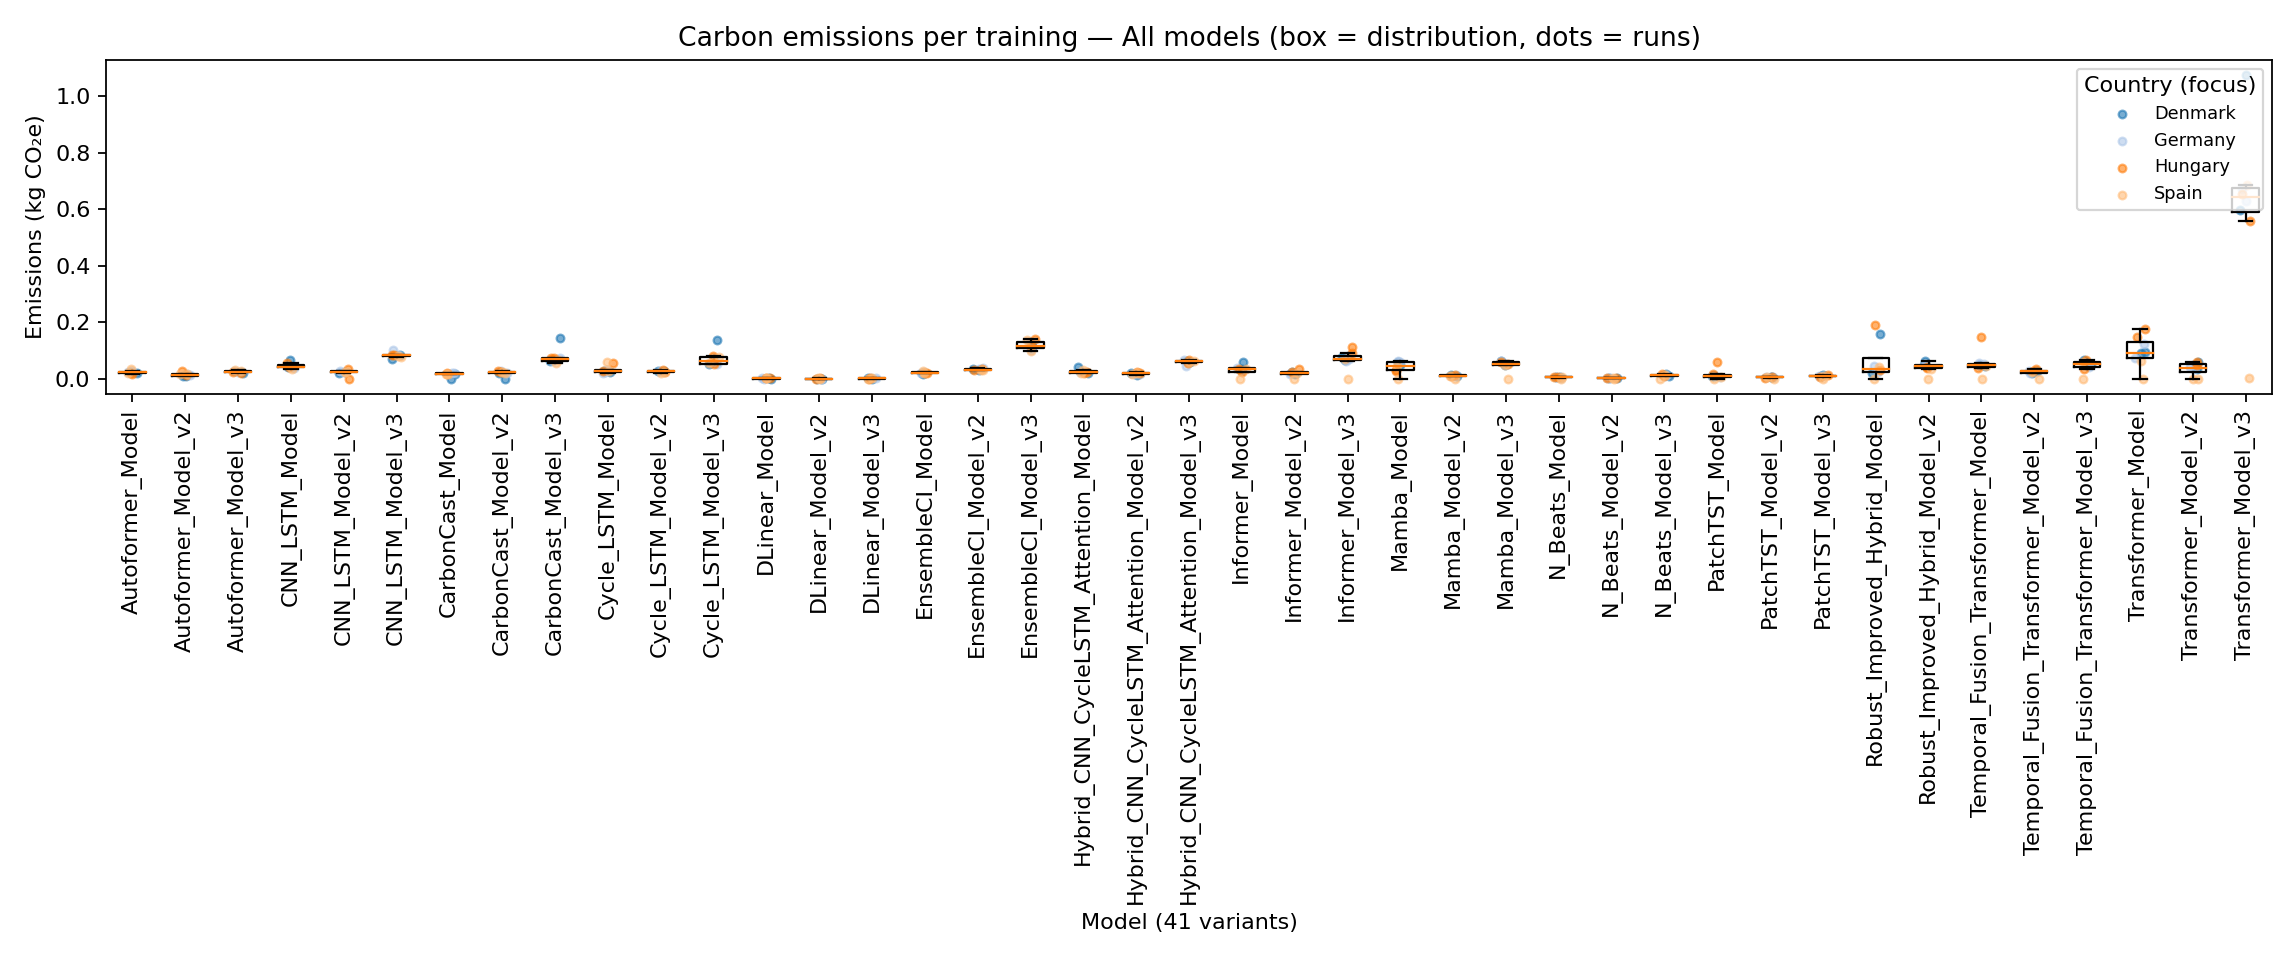
\includegraphics[width=0.95\linewidth]{../Results/Benchmark/boxplot_emissions_all_models.png}
  \caption{Emissions distribution across models.}
  \label{fig:emissions_boxplots}
\end{figure}

\begin{figure}[t]
  \centering
  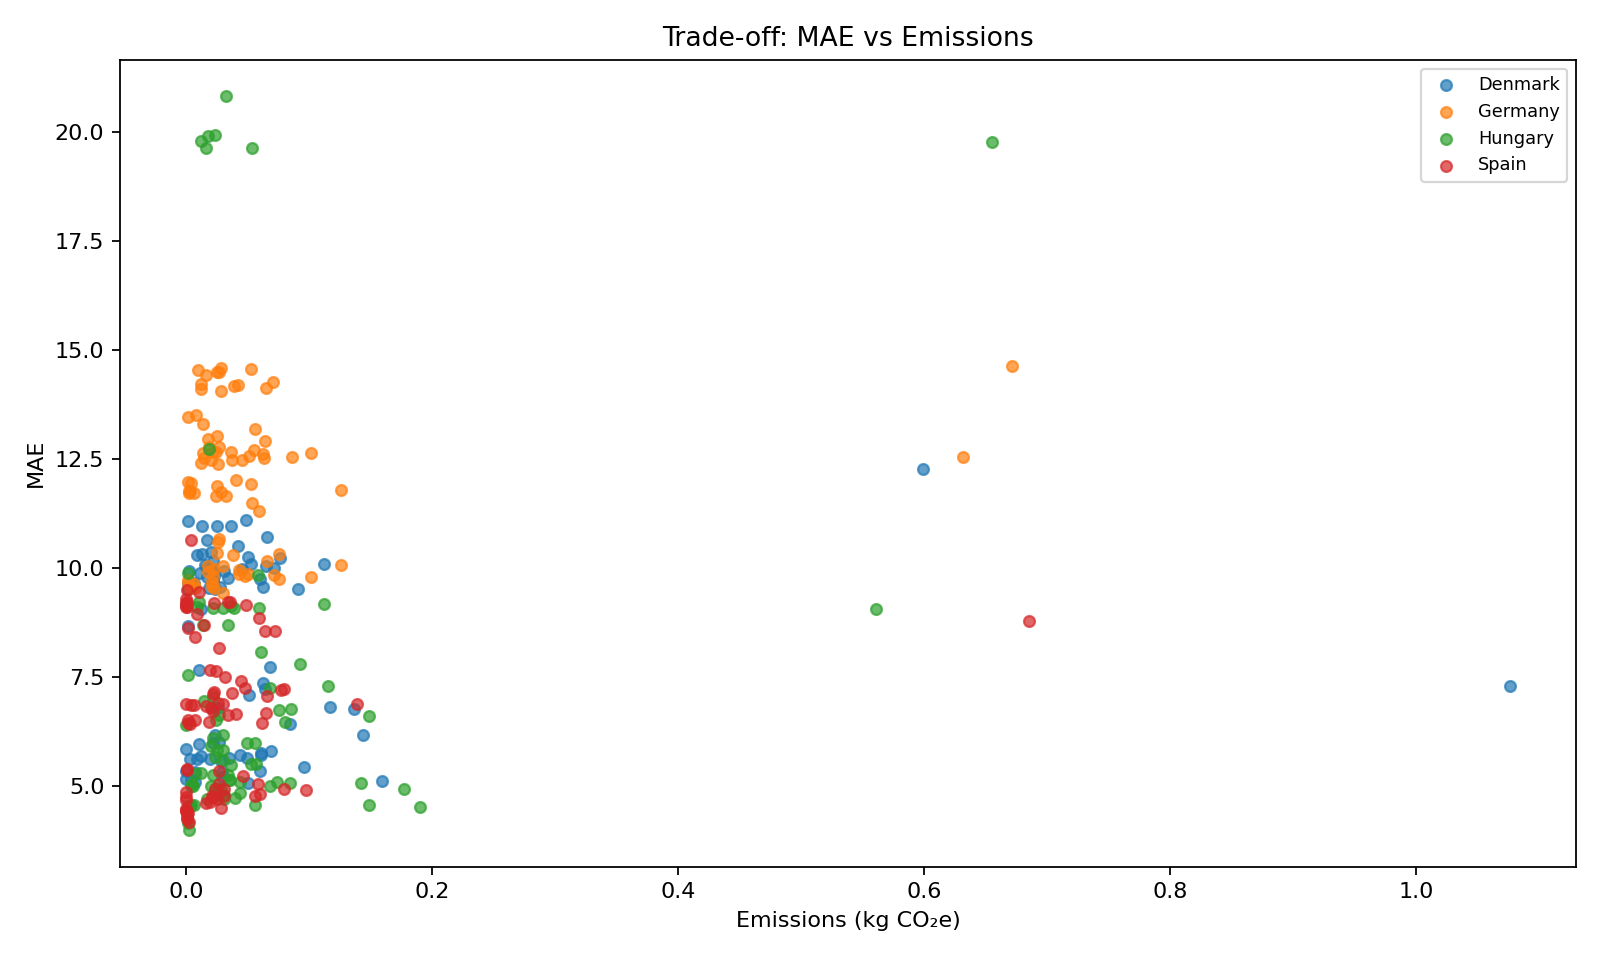
\includegraphics[width=0.95\linewidth]{../Results/Benchmark/tradeoff_mae_vs_emissions.png}
  \caption{MAE vs Emissions trade-off.}
  \label{fig:tradeoff}
\end{figure}

% Additional figures: Emissions by country (grid)
\begin{figure*}[t]
  \centering
  \subfloat[Denmark]{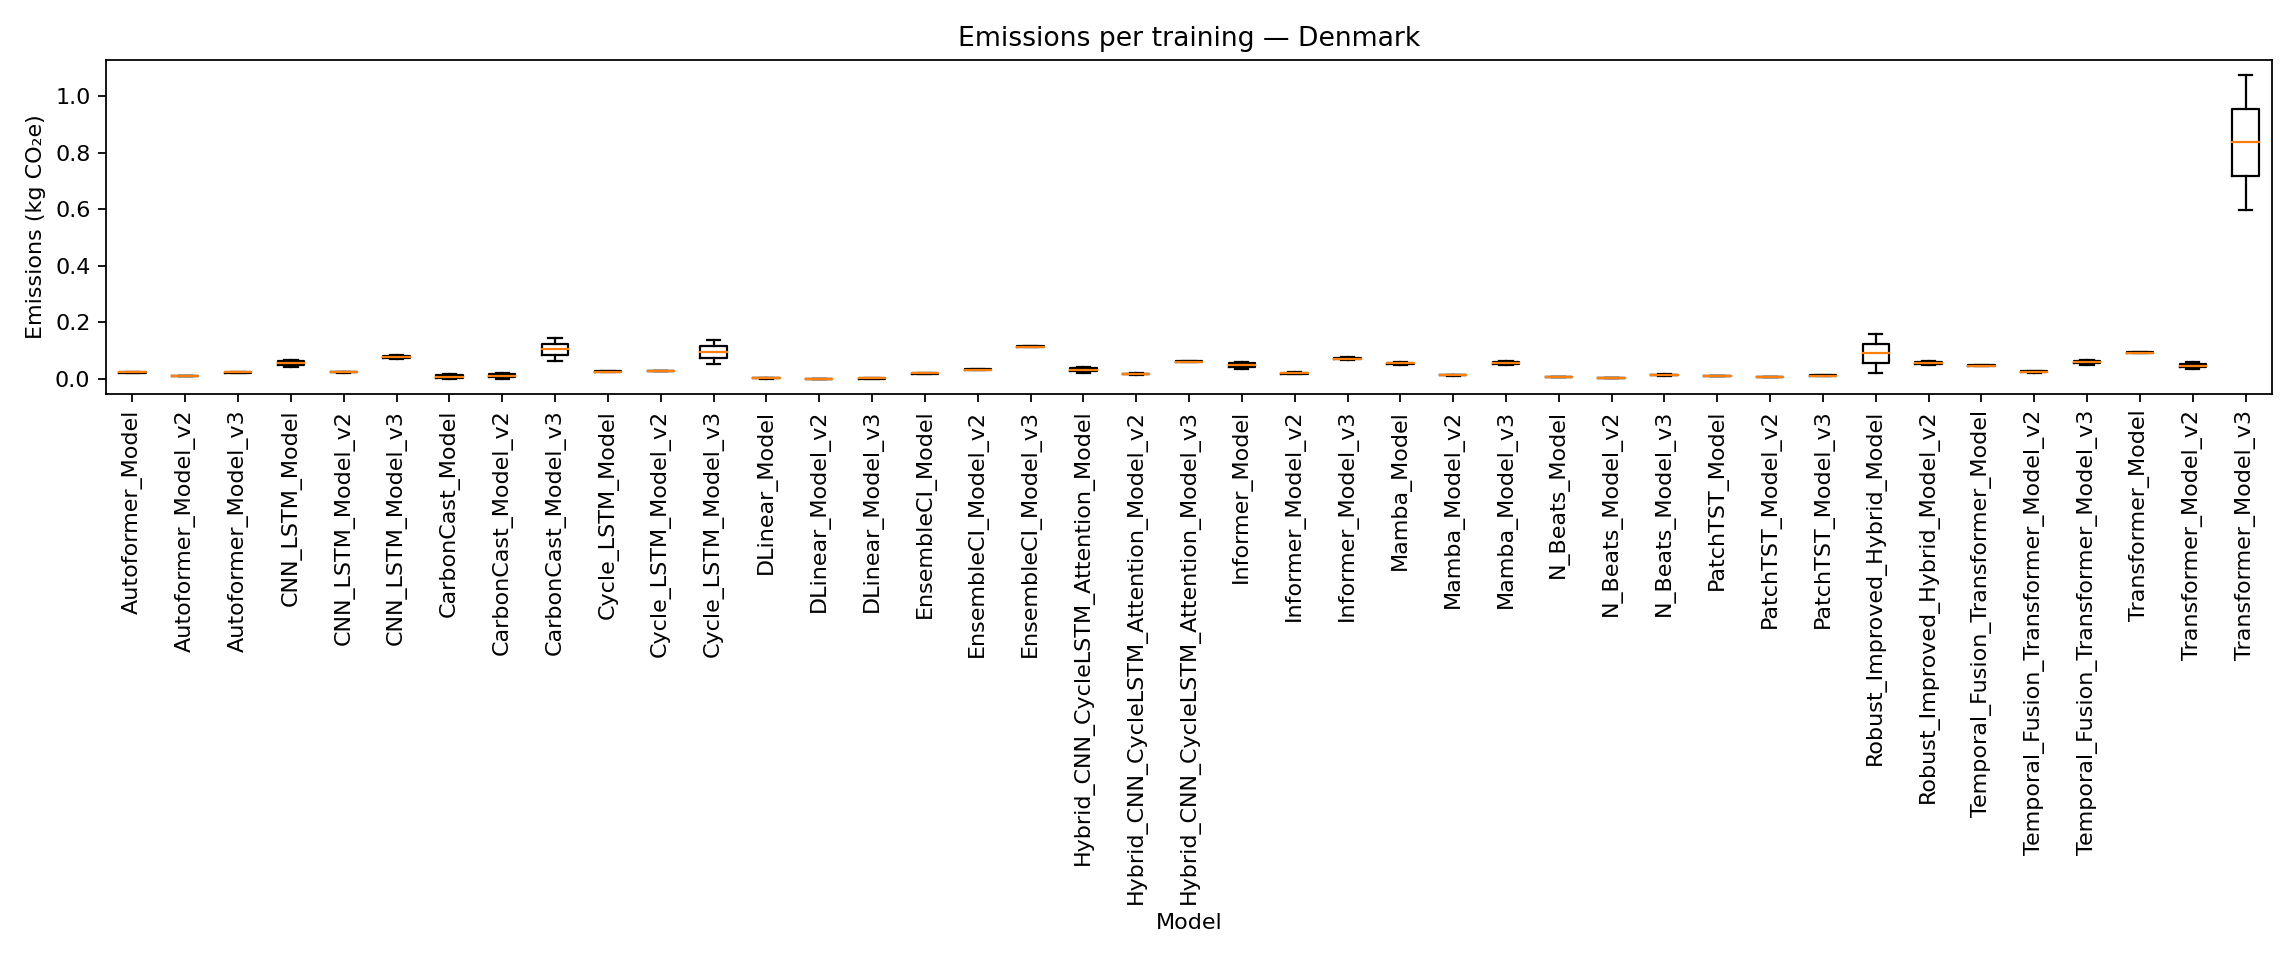
\includegraphics[width=0.48\textwidth]{../Results/Benchmark/boxplot_emissions_Denmark.png}}\hfill
  \subfloat[Germany]{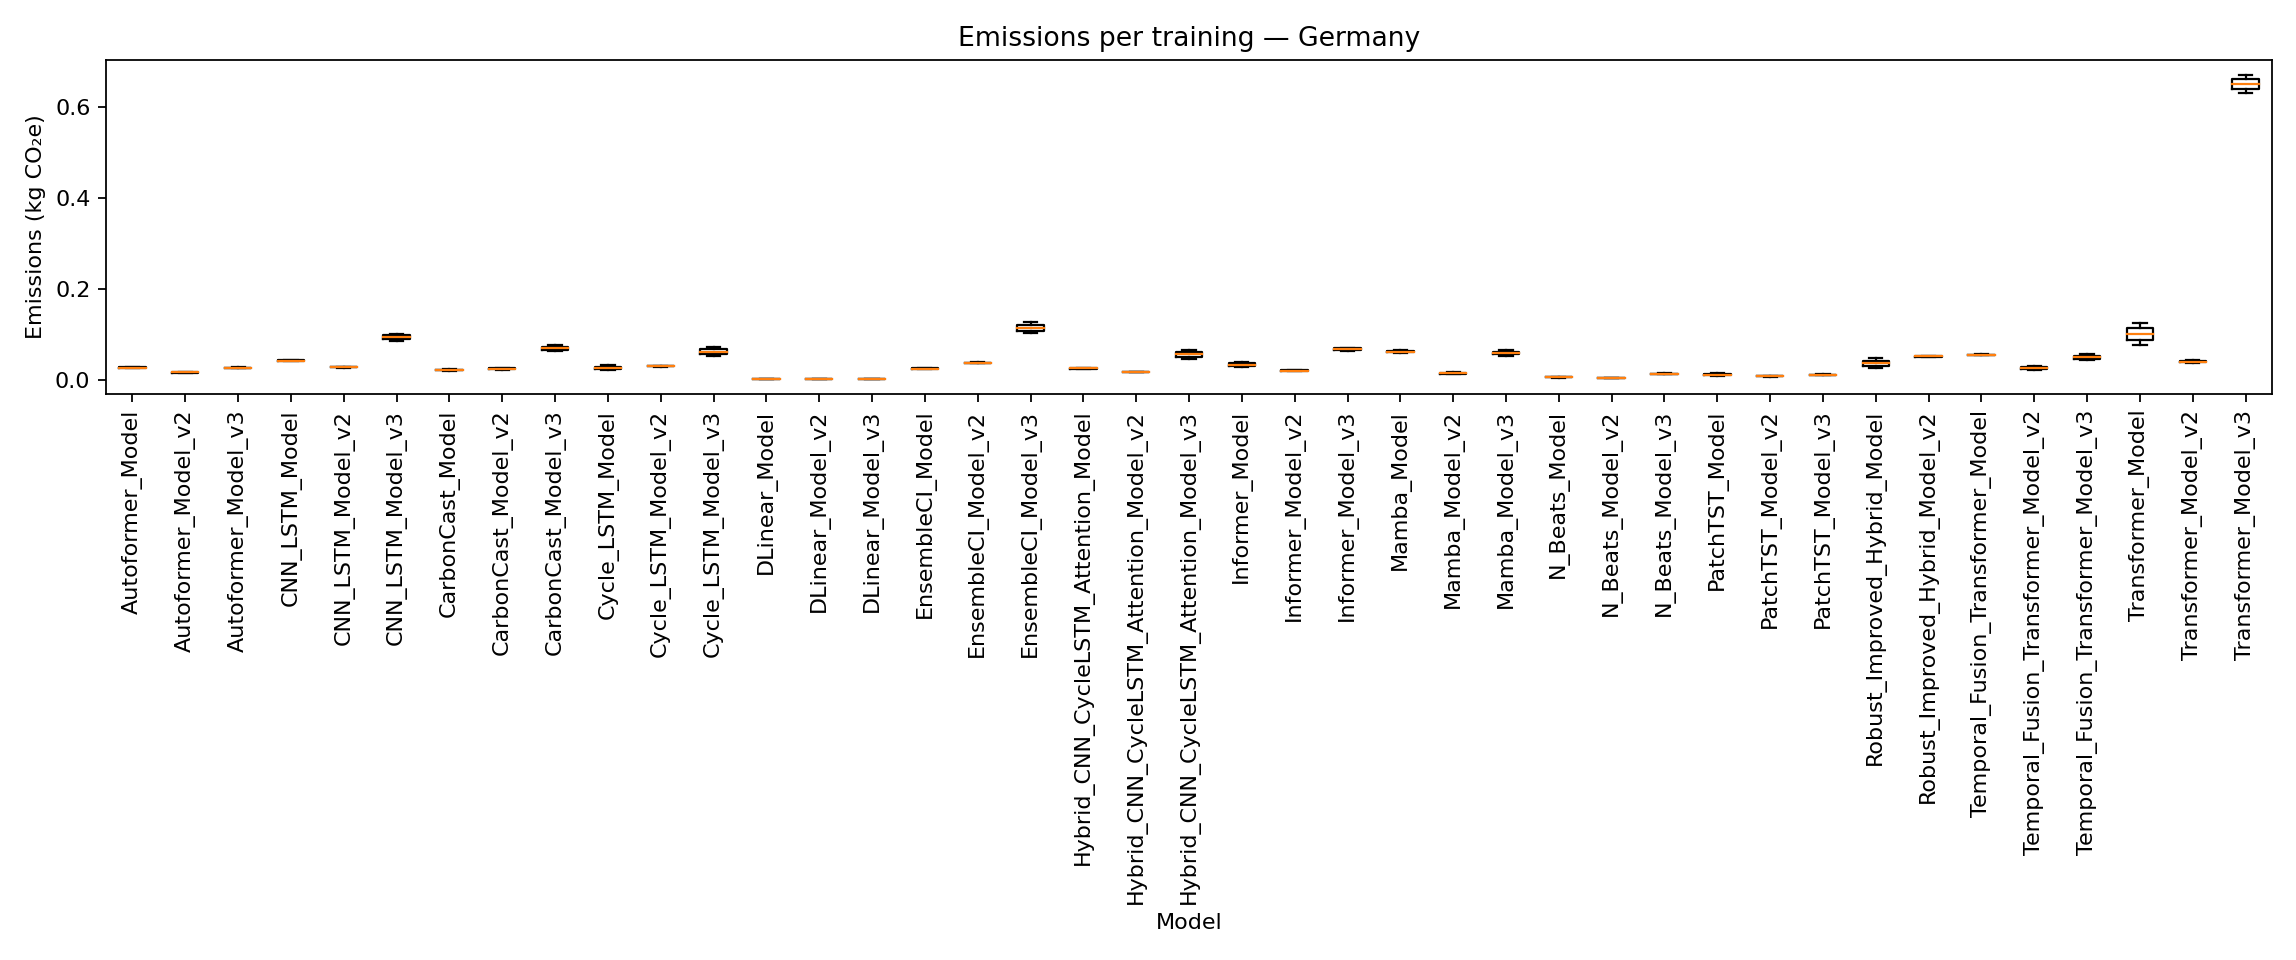
\includegraphics[width=0.48\textwidth]{../Results/Benchmark/boxplot_emissions_Germany.png}}\\
  \subfloat[Hungary]{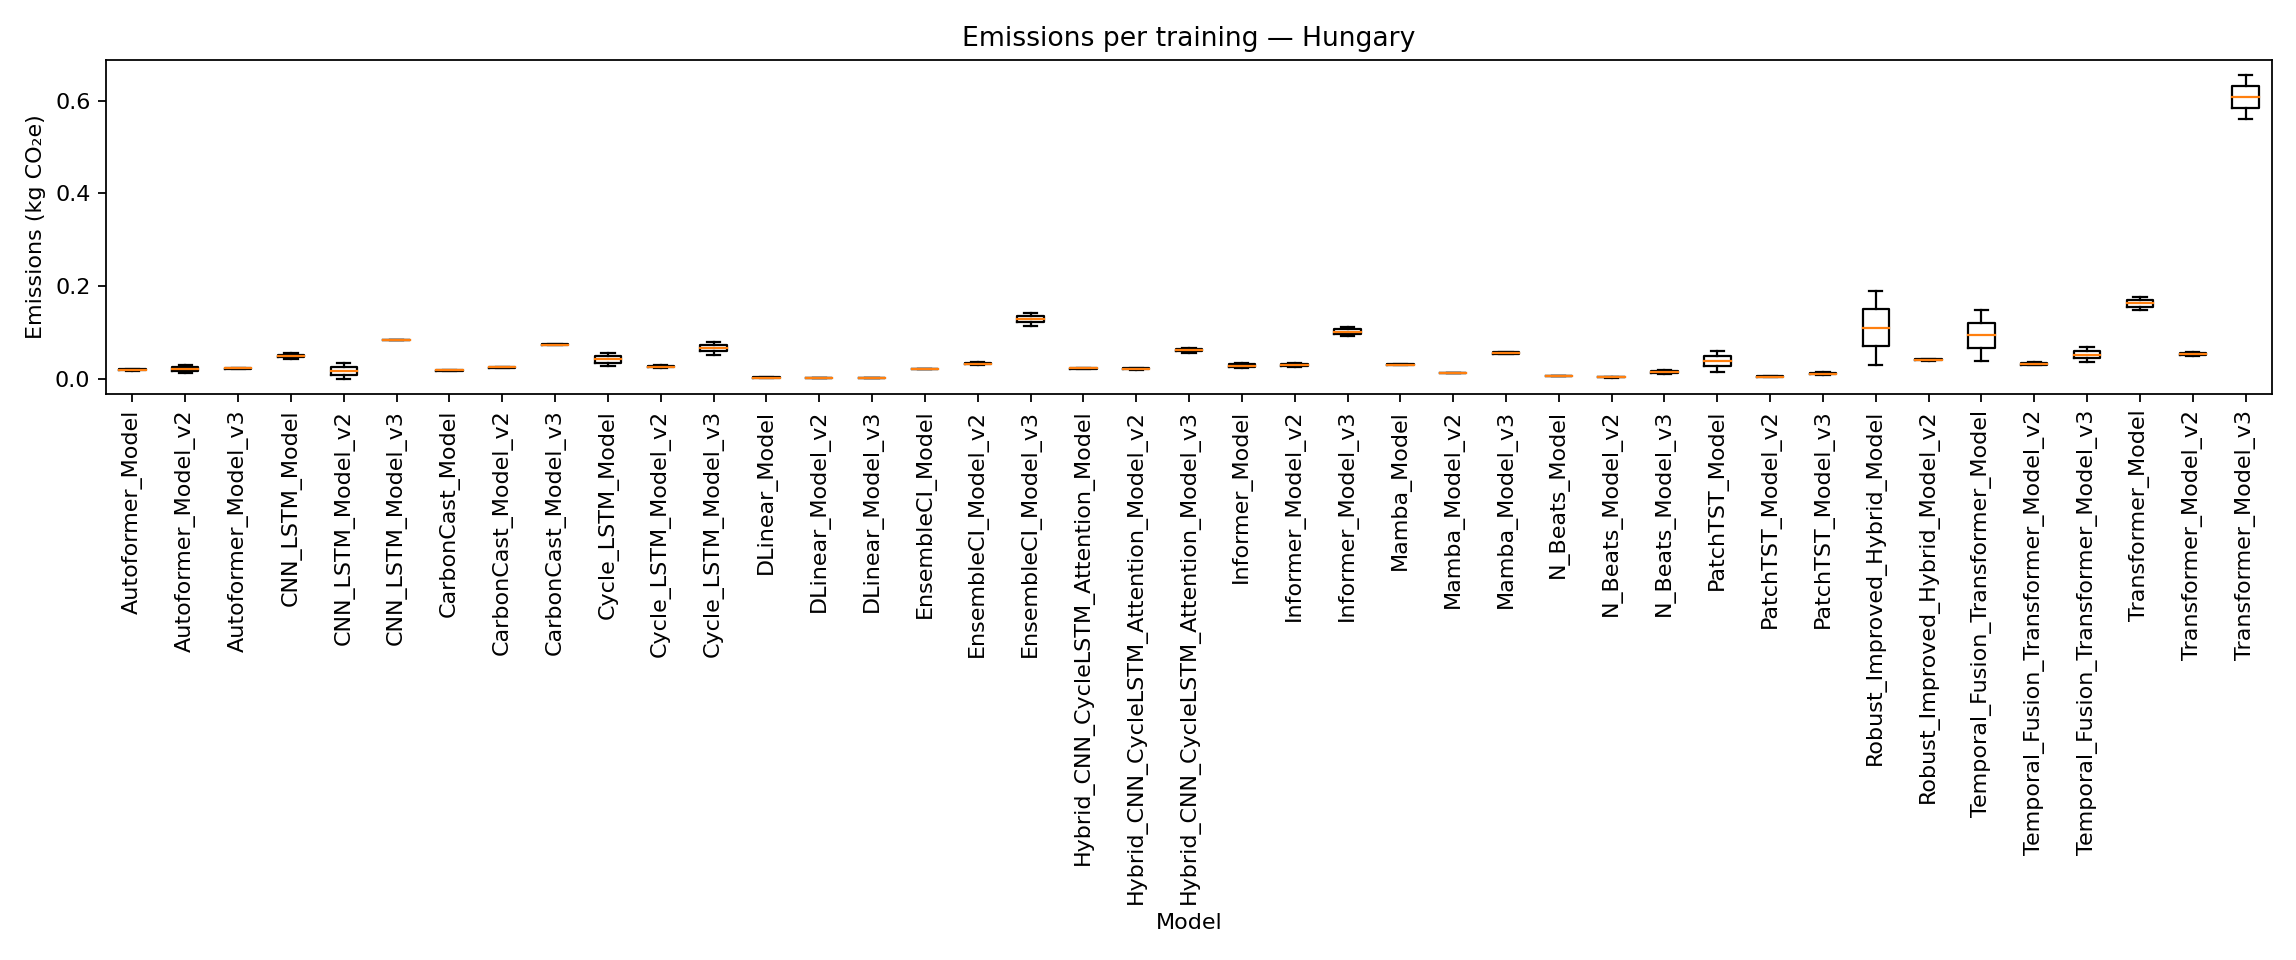
\includegraphics[width=0.48\textwidth]{../Results/Benchmark/boxplot_emissions_Hungary.png}}\hfill
  \subfloat[Spain]{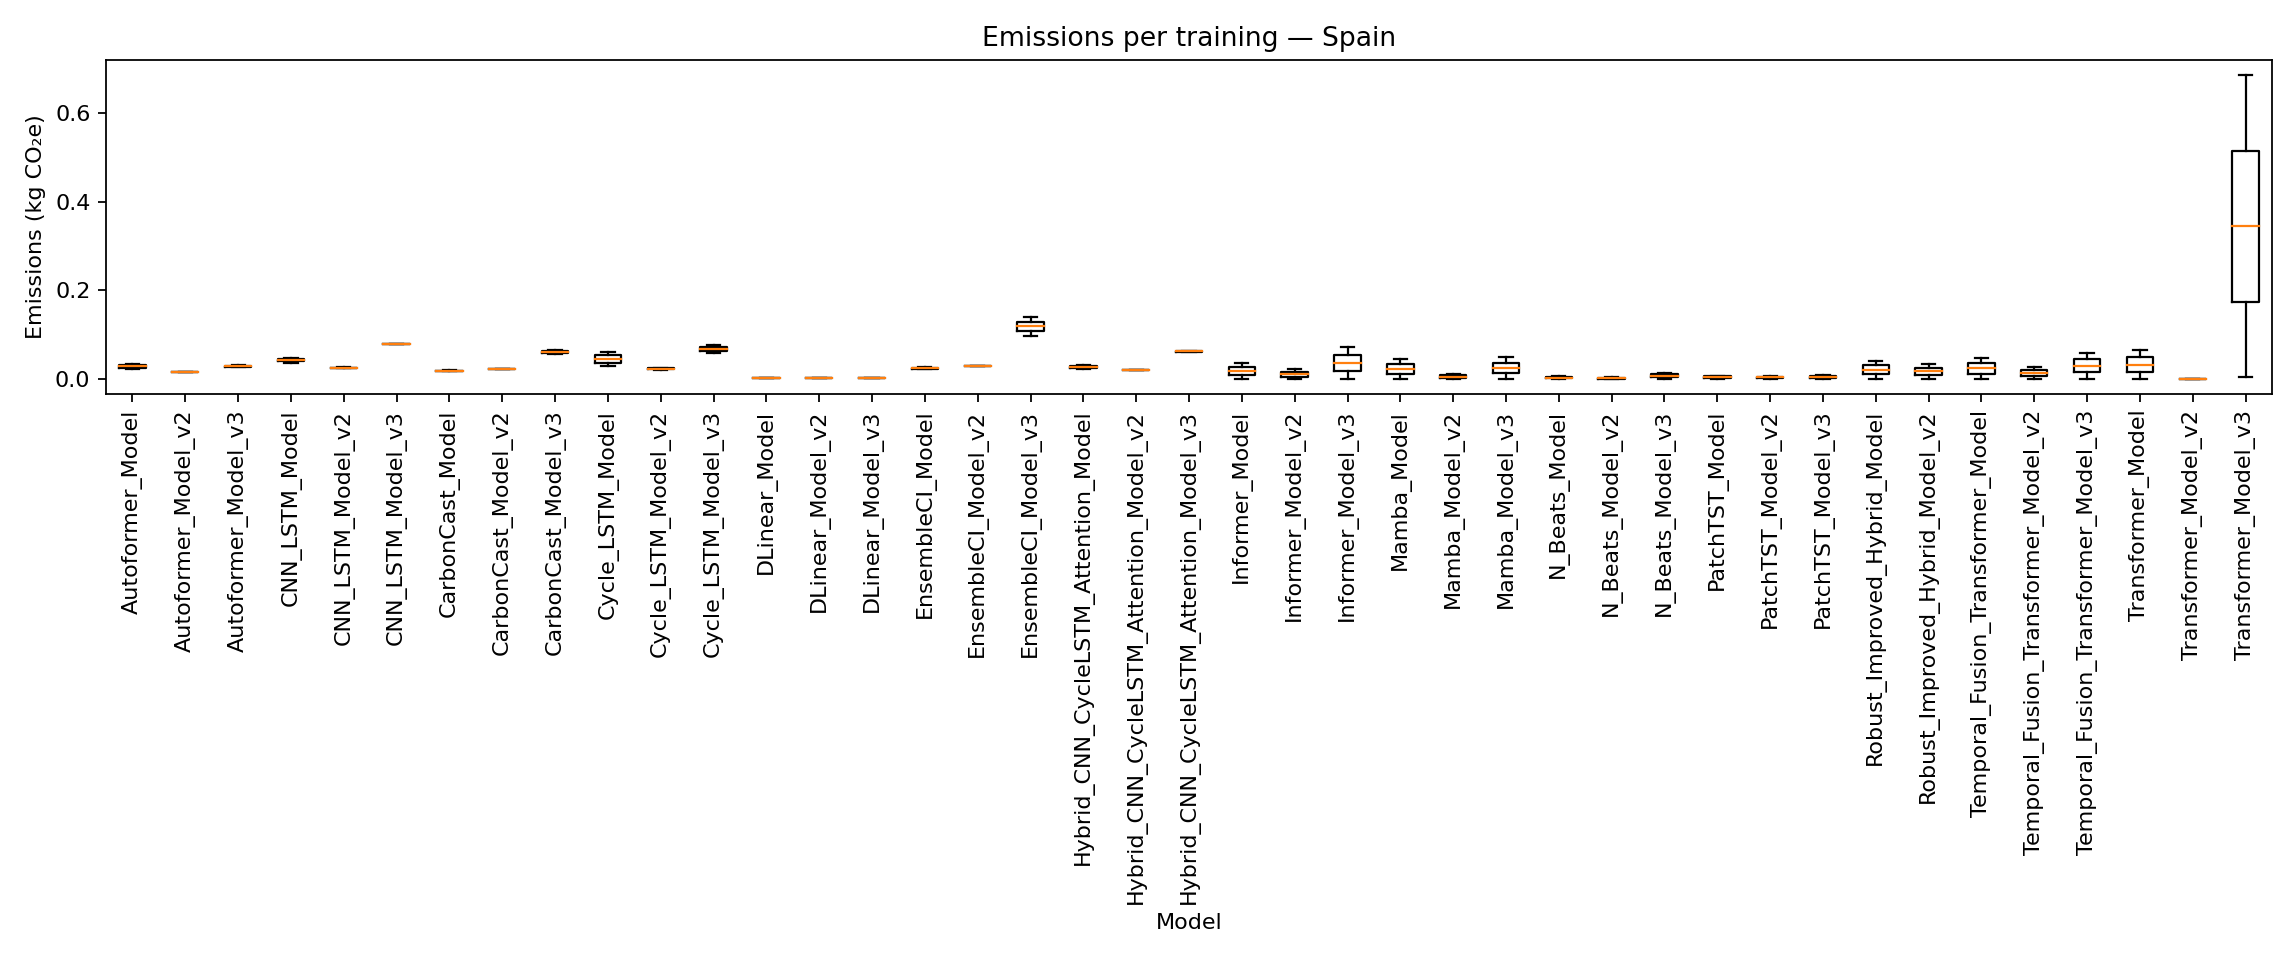
\includegraphics[width=0.48\textwidth]{../Results/Benchmark/boxplot_emissions_Spain.png}}
  \caption{Per-country emissions distributions across models.}
  \label{fig:per_country_emissions}
\end{figure*}

% Additional figures: Heatmaps and Top-10 leaderboard
\begin{figure*}[t]
  \centering
  \subfloat[Mean MAE (summer)]{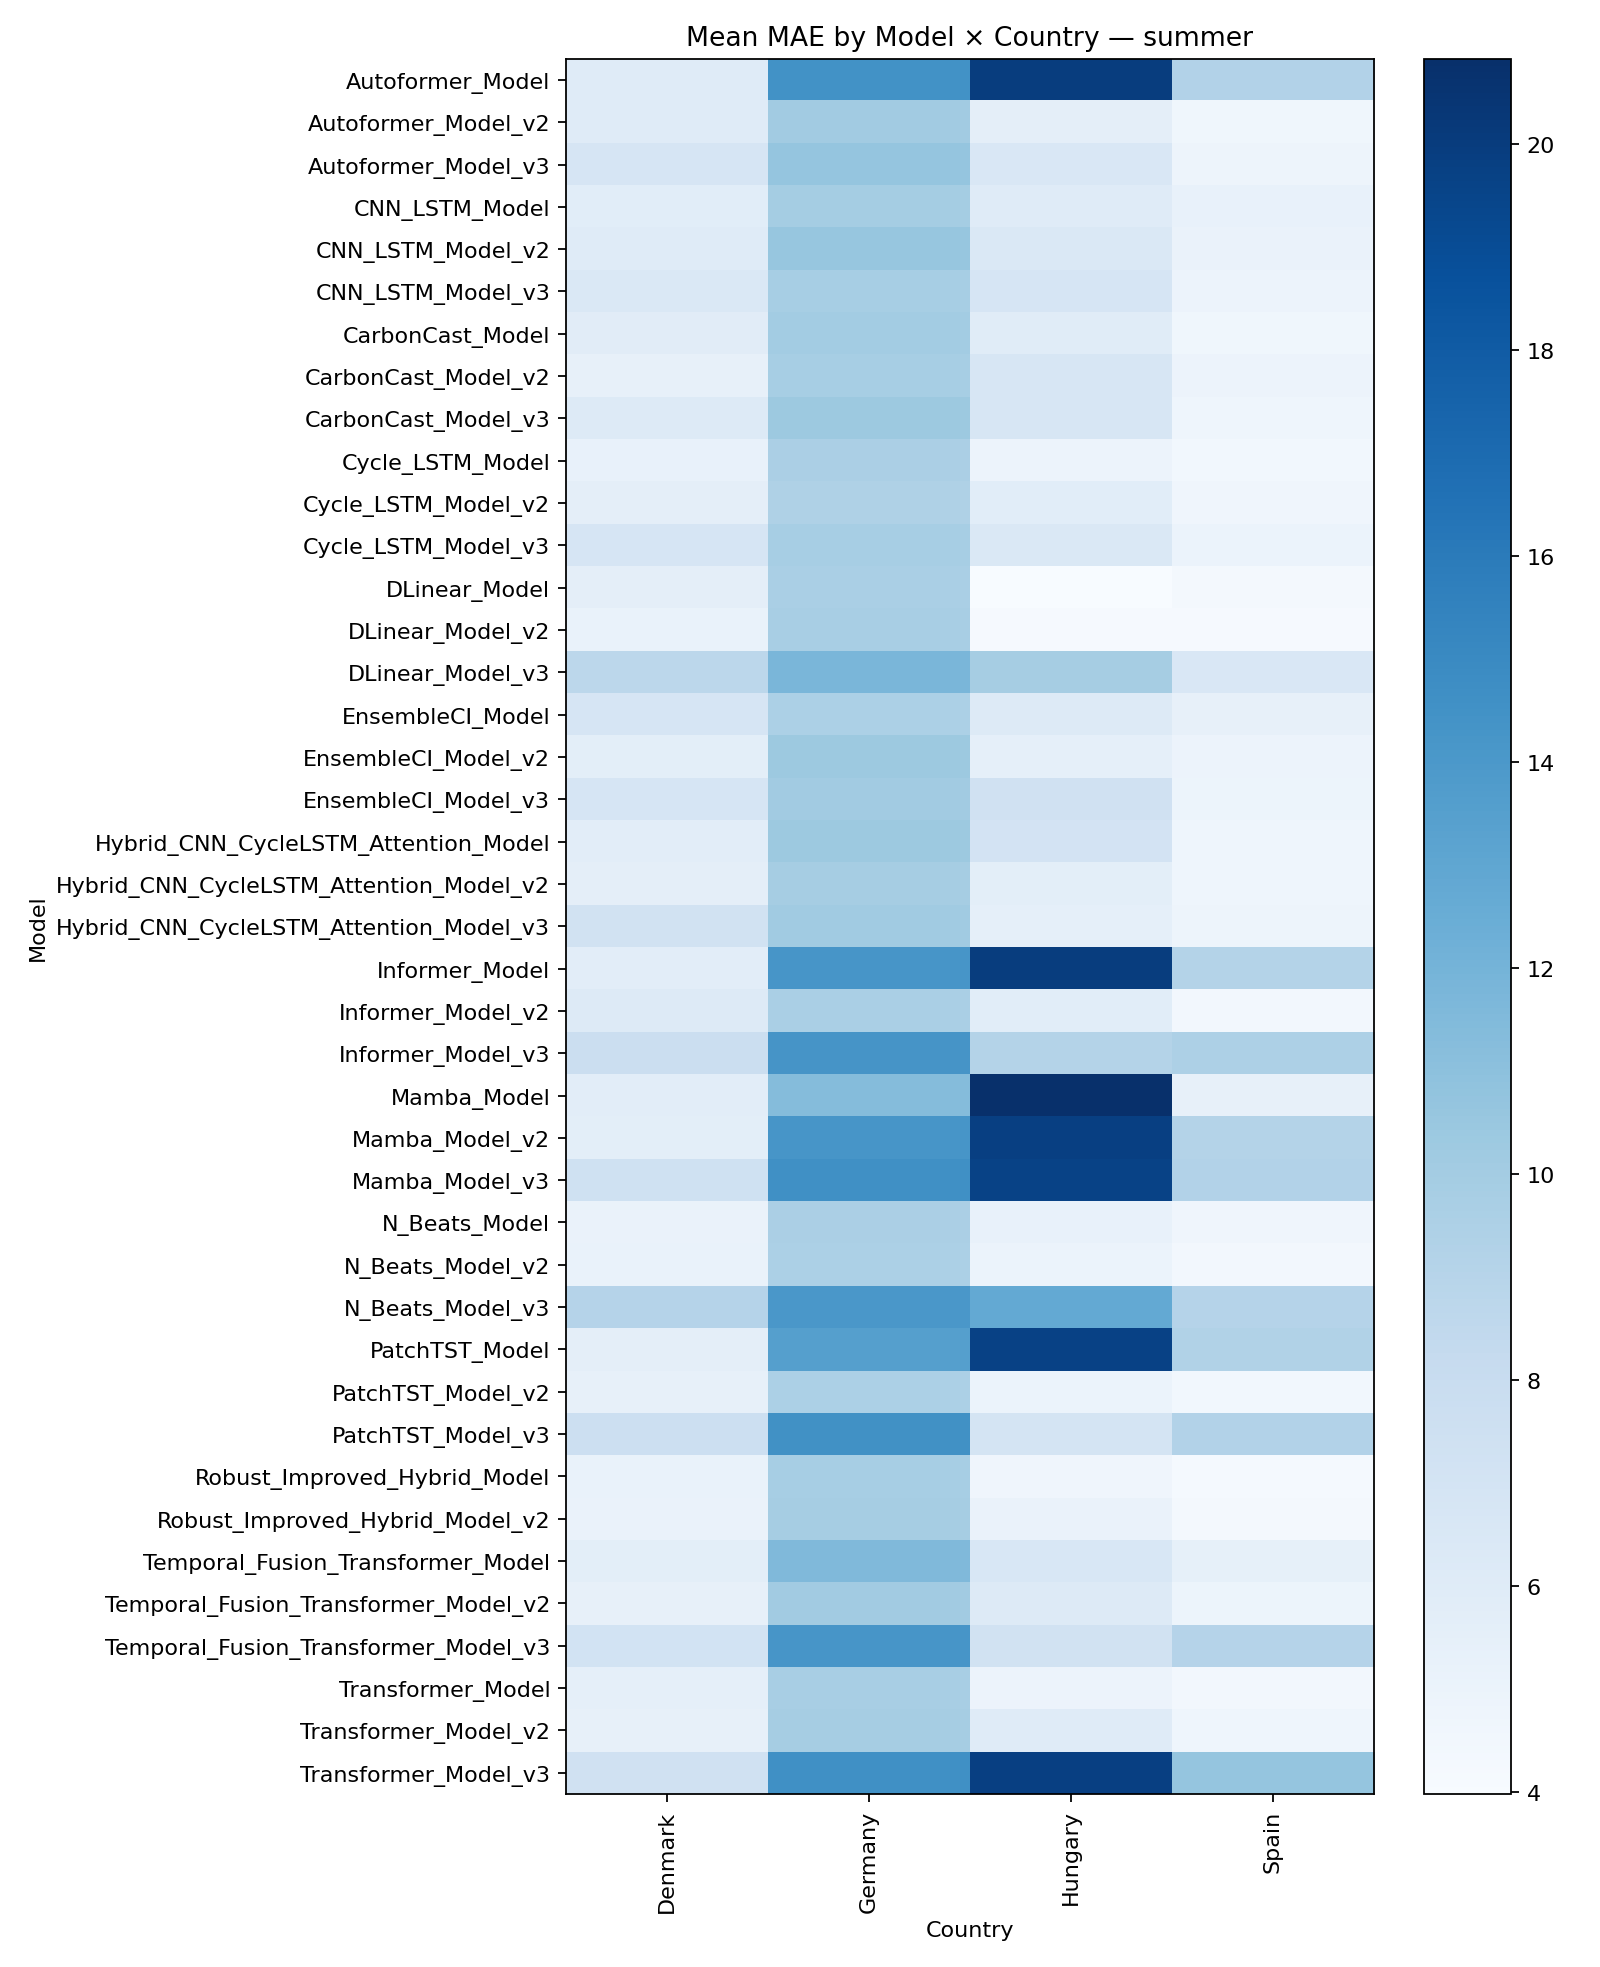
\includegraphics[width=0.48\textwidth]{../Results/Benchmark/heatmap_mean_mae_summer.png}}\hfill
  \subfloat[Mean MAE (winter)]{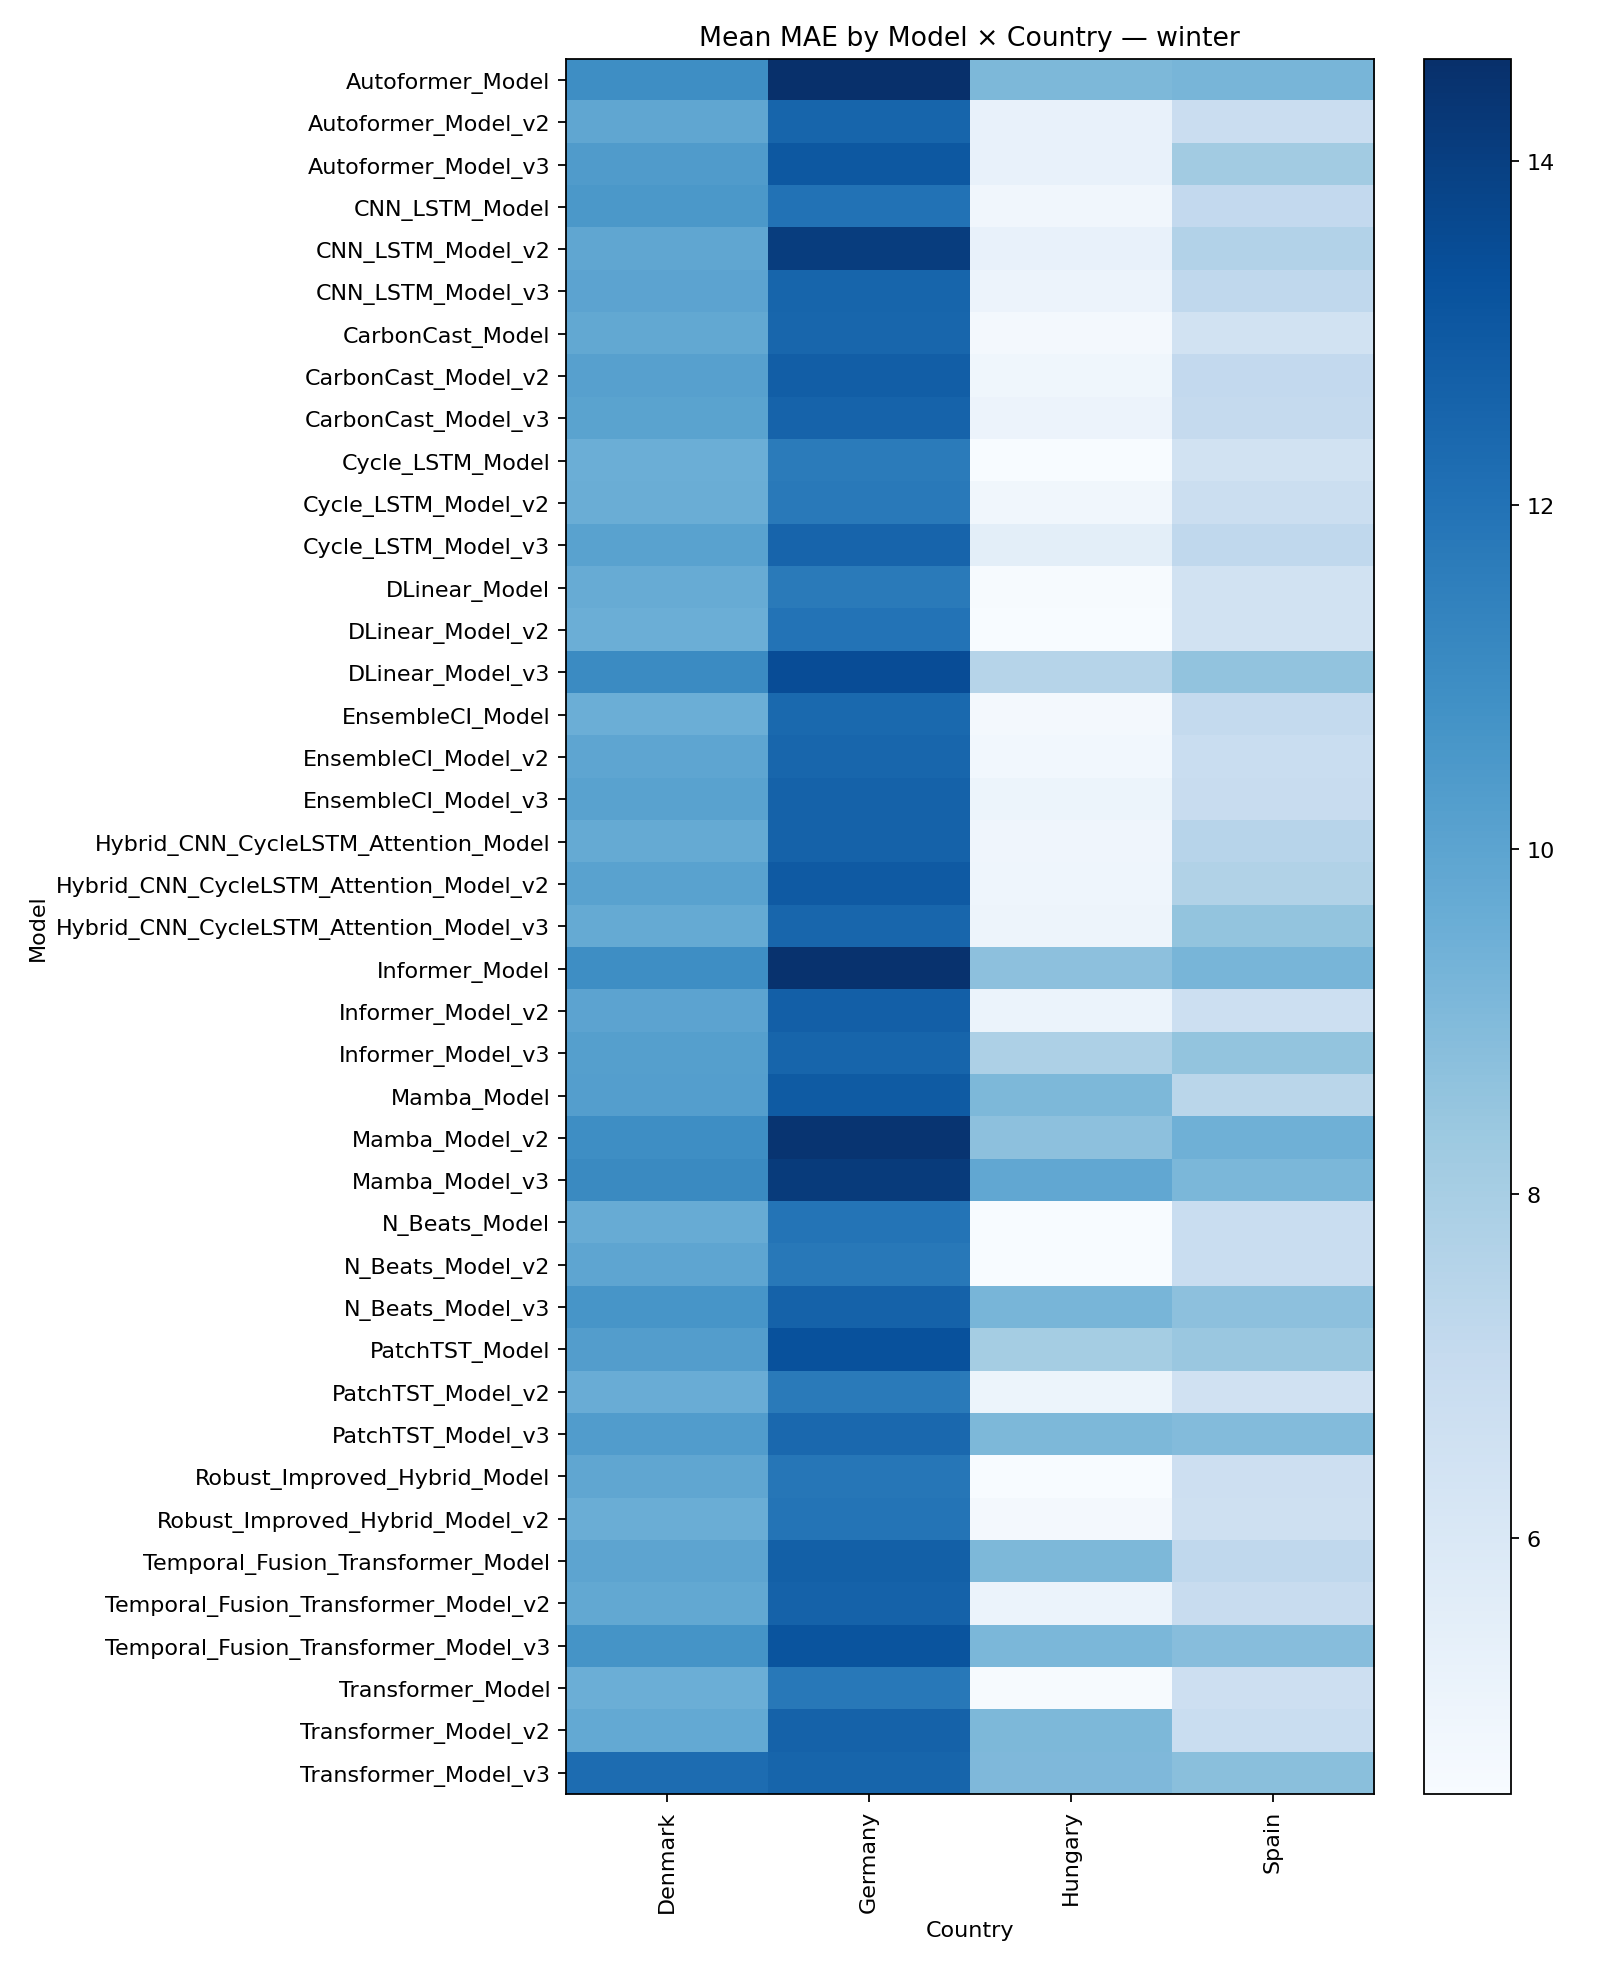
\includegraphics[width=0.48\textwidth]{../Results/Benchmark/heatmap_mean_mae_winter.png}}
  \caption{Heatmaps of mean MAE by model and country.}
  \label{fig:heatmaps_mae}
\end{figure*}

\begin{figure*}[t]
  \centering
  \subfloat[Mean emissions (summer)]{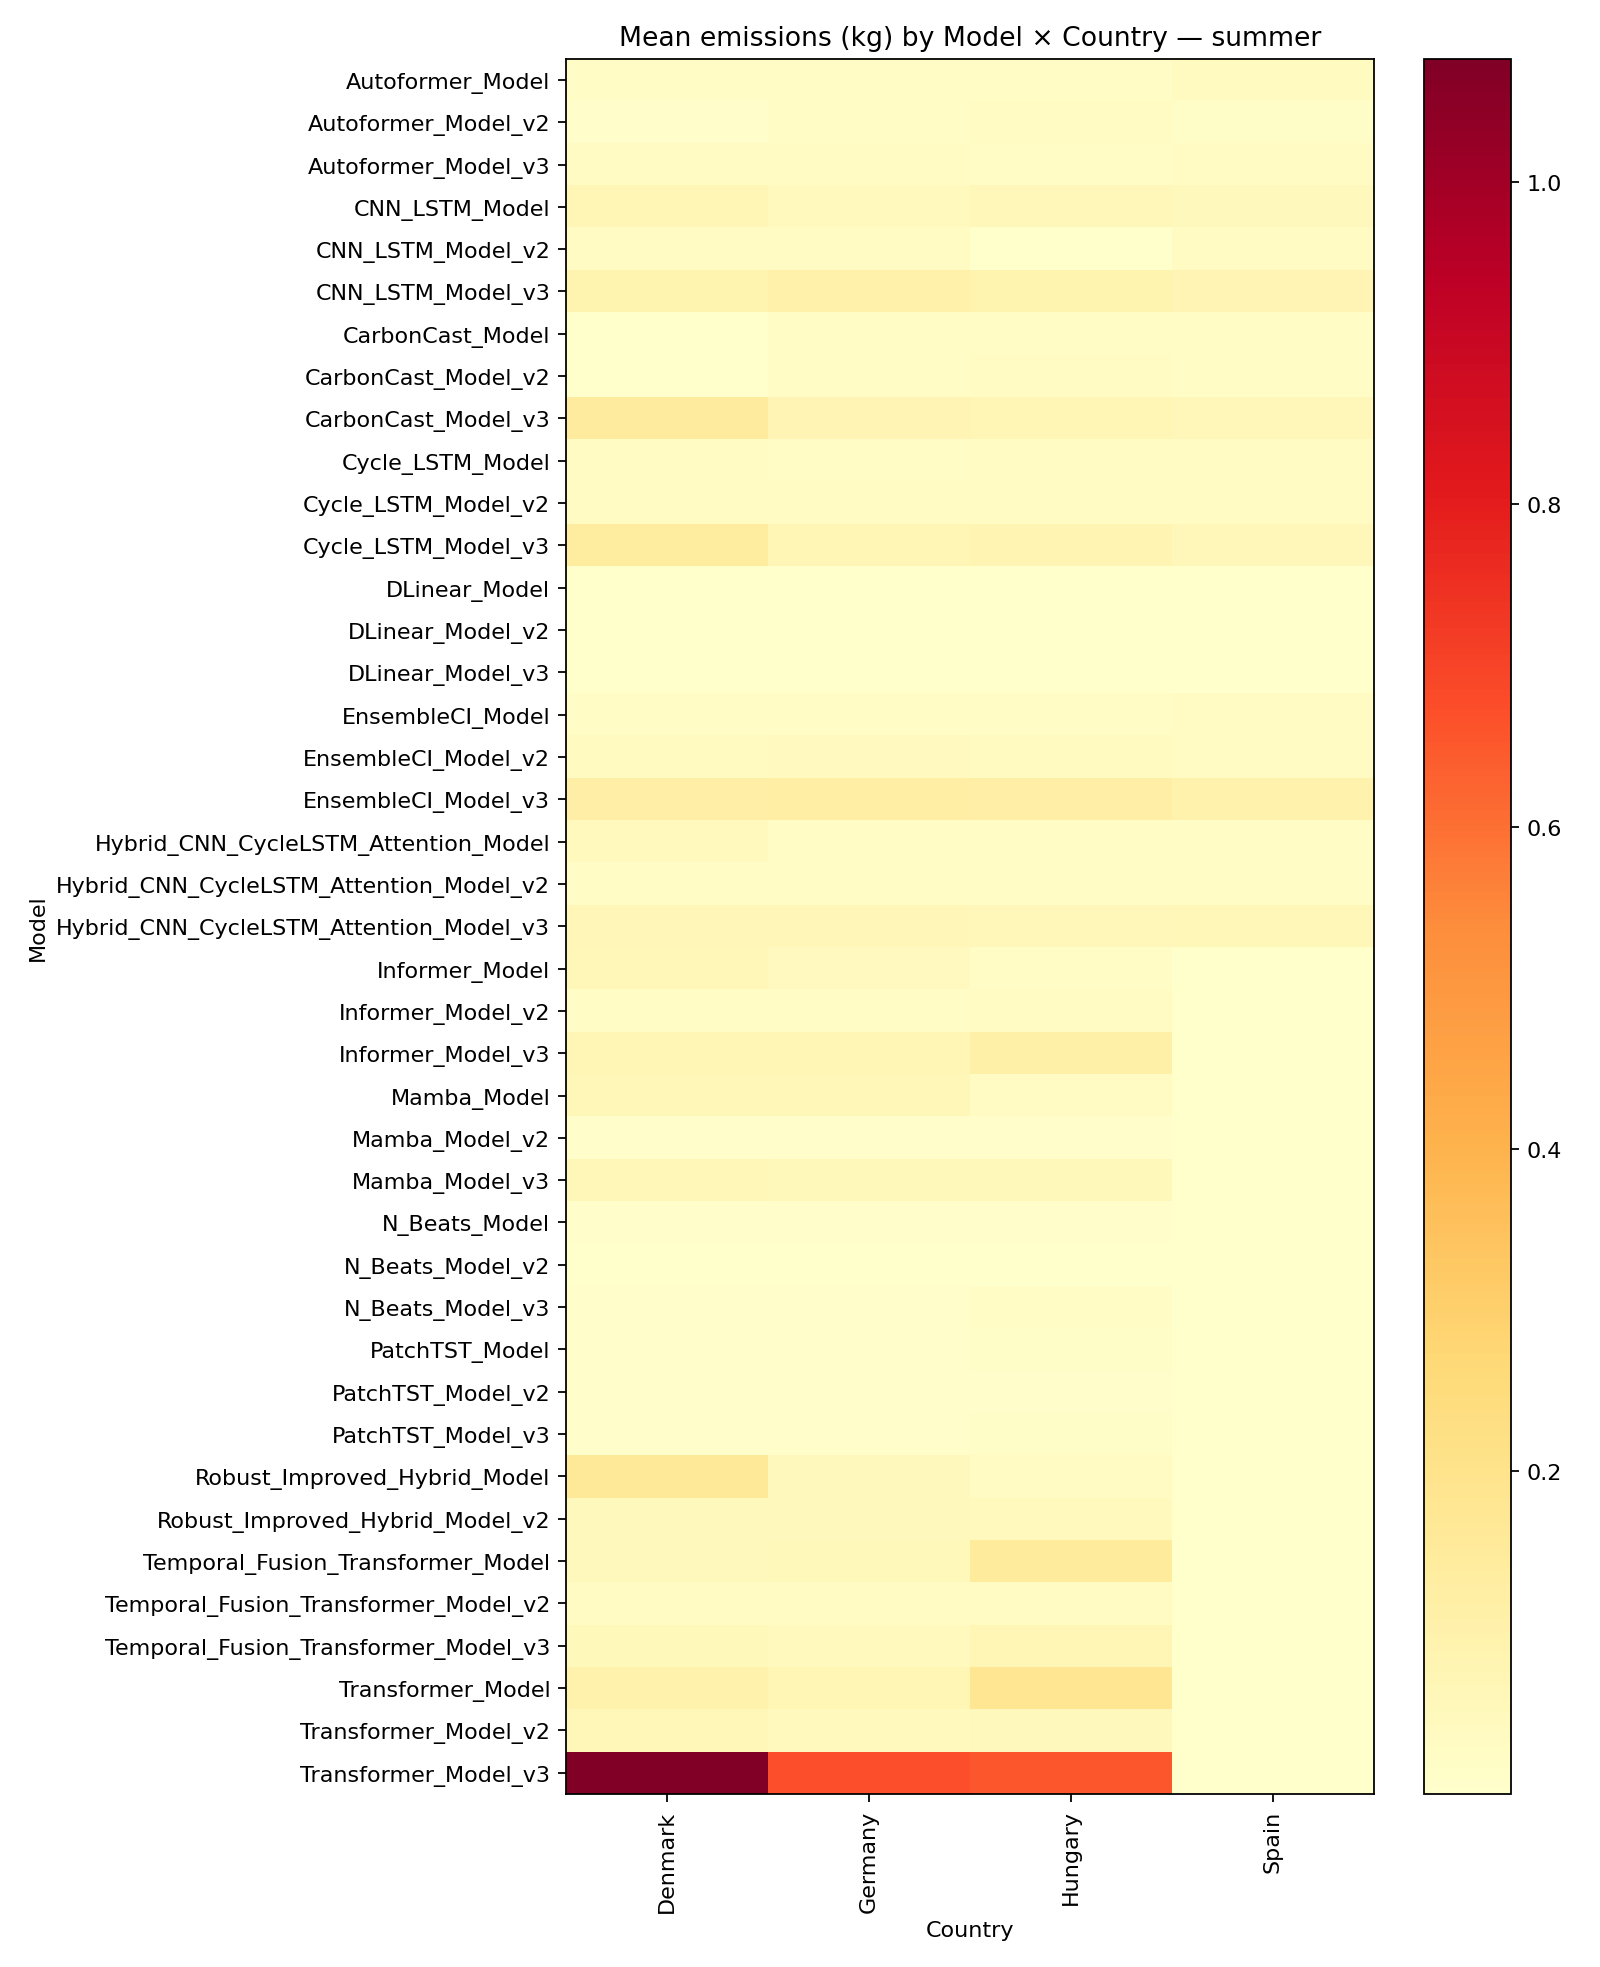
\includegraphics[width=0.48\textwidth]{../Results/Benchmark/heatmap_mean_emissions_summer.png}}\hfill
  \subfloat[Mean emissions (winter)]{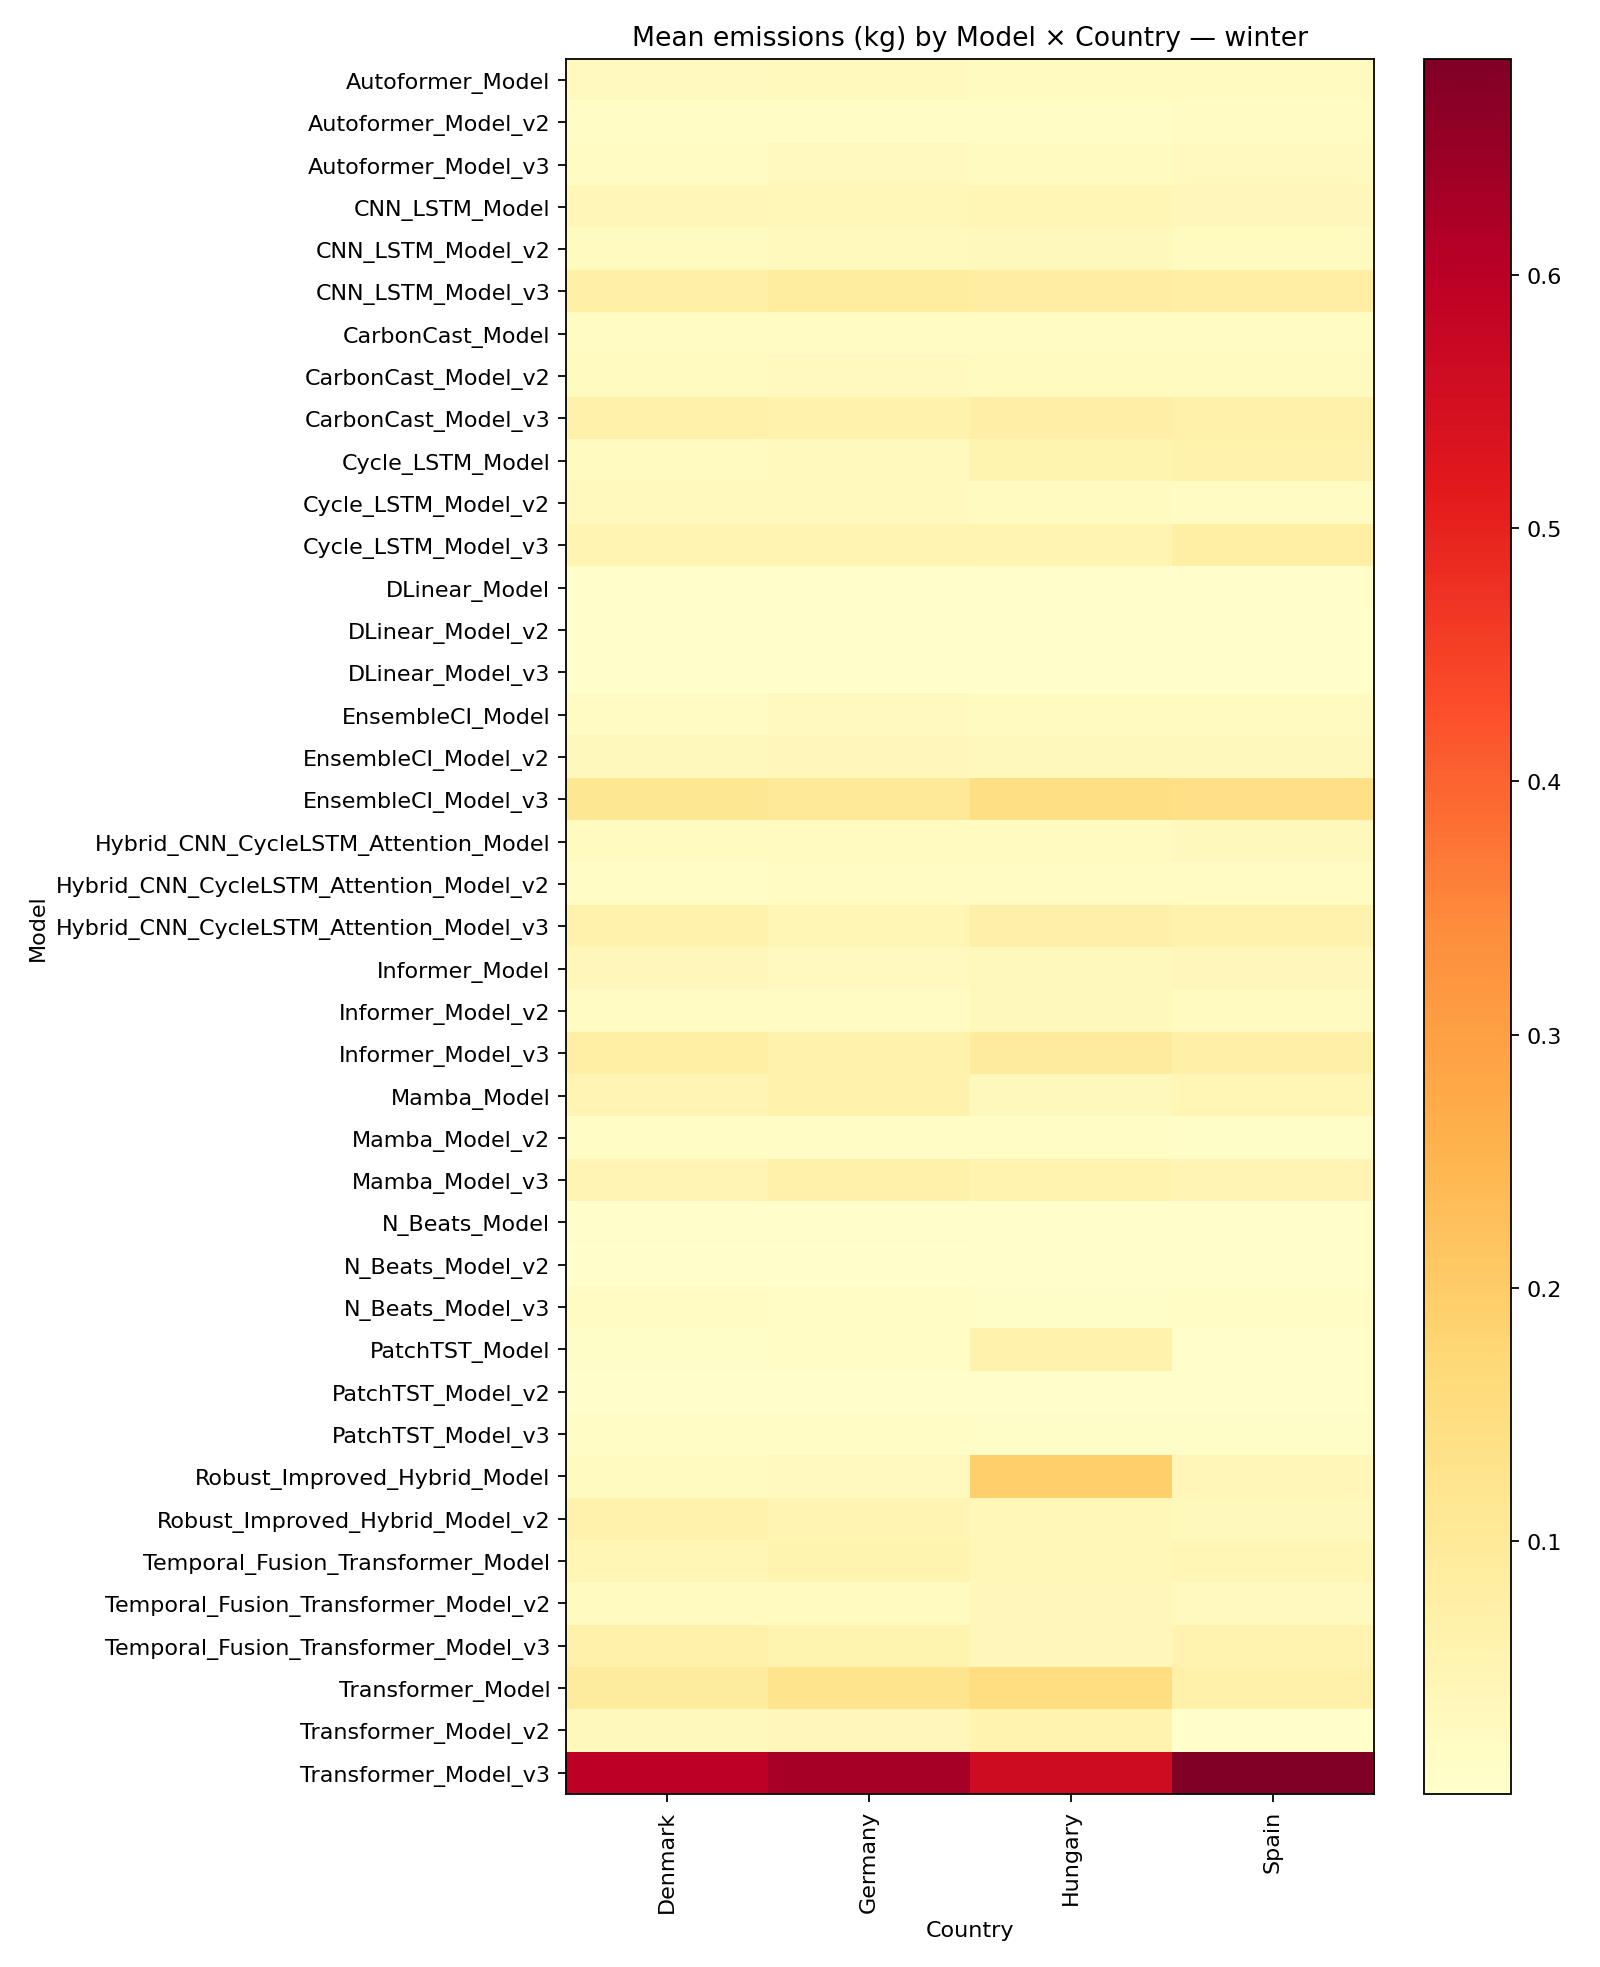
\includegraphics[width=0.48\textwidth]{../Results/Benchmark/heatmap_mean_emissions_winter.png}}
  \caption{Heatmaps of mean emissions (kg CO\textsubscript{2}e) by model and country.}
  \label{fig:heatmaps_emissions}
\end{figure*}

\begin{figure}[t]
  \centering
  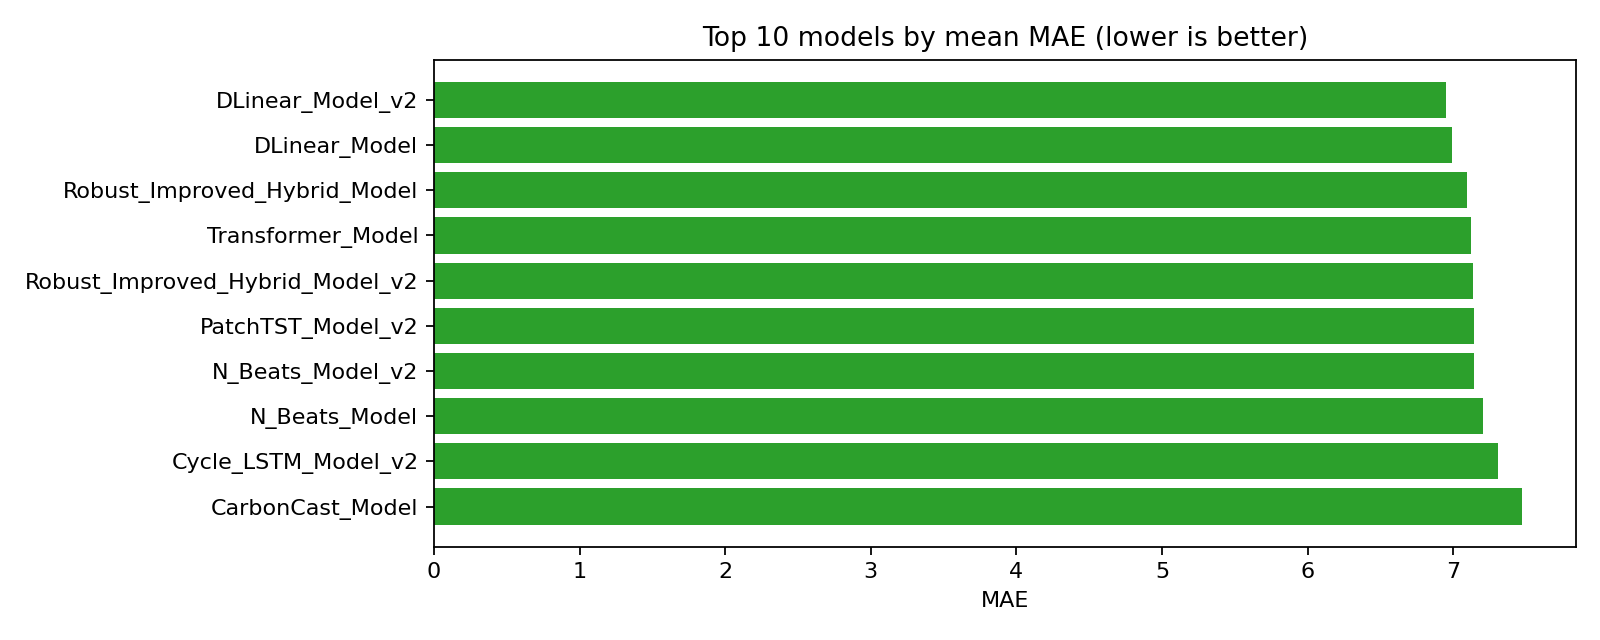
\includegraphics[width=0.95\linewidth]{../Results/Benchmark/top10_mae.png}
  \caption{Global Top-10 MAE leaderboard across slices.}
  \label{fig:top10_mae}
\end{figure}

% Low-carbon leaders table (generated)
\begin{table}[t]
  \centering
  \caption{Low-carbon leaders (best MAE with emissions $\leq$ 0.10 kg CO\textsubscript{2}e) by slice.}
  \label{tab:low_carbon_leaders}
  % Generated by Paper/generate\_tables.py using emissions\_aggregated.csv
  \begin{tabular}{l l r r}
\toprule
Slice & Model & MAE & Emissions (kg) \\
\midrule
Denmark Summer & Robust\_Improved\_Hybrid\_Model\_v2 & 5.053 & 0.050 \\
Denmark Winter & Transformer\_Model & 9.515 & 0.091 \\
Germany Summer & Cycle\_LSTM\_Model\_v2 & 9.433 & 0.030 \\
Germany Winter & Cycle\_LSTM\_Model & 11.640 & 0.025 \\
Hungary Summer & DLinear\_Model & 3.979 & 0.002 \\
Hungary Winter & DLinear\_Model\_v2 & 4.528 & 0.002 \\
Spain Summer & DLinear\_Model\_v2 & 4.162 & 0.002 \\
Spain Winter & DLinear\_Model & 6.422 & 0.003 \\
\bottomrule
\end{tabular}

\end{table}

% Pareto leaders table (generated)
\begin{table}[t]
  \centering
  \caption{Pareto leaders by slice (minimizing MAE and emissions).}
  \label{tab:pareto_leaders}
  \begin{tabular}{l l r r}
\toprule
Slice & Model & MAE & Emissions (kg) \\
\midrule
Denmark Summer & Robust\_Improved\_Hybrid\_Model\_v2 & 5.053 & 0.050 \\
Denmark Summer & N\_Beats\_Model & 5.072 & 0.007 \\
Denmark Summer & N\_Beats\_Model\_v2 & 5.134 & 0.004 \\
Denmark Winter & Transformer\_Model & 9.515 & 0.091 \\
Denmark Winter & Cycle\_LSTM\_Model & 9.518 & 0.023 \\
Denmark Winter & DLinear\_Model\_v2 & 9.519 & 0.001 \\
Germany Summer & Cycle\_LSTM\_Model\_v2 & 9.433 & 0.030 \\
Germany Summer & PatchTST\_Model\_v2 & 9.533 & 0.007 \\
Germany Summer & N\_Beats\_Model\_v2 & 9.545 & 0.003 \\
Germany Winter & Cycle\_LSTM\_Model & 11.649 & 0.028 \\
Germany Winter & DLinear\_Model & 11.710 & 0.002 \\
Germany Winter & PatchTST\_Model\_v2 & 11.710 & 0.007 \\
Hungary Summer & DLinear\_Model & 3.979 & 0.002 \\
Hungary Summer & DLinear\_Model\_v2 & 4.134 & 0.002 \\
Hungary Summer & CNN\_LSTM\_Model\_v2 & 6.398 & 0.000 \\
Hungary Winter & Robust\_Improved\_Hybrid\_Model & 4.514 & 0.190 \\
Hungary Winter & DLinear\_Model\_v2 & 4.528 & 0.002 \\
Hungary Winter & DLinear\_Model\_v3 & 7.535 & 0.001 \\
Spain Summer & DLinear\_Model\_v2 & 4.162 & 0.002 \\
Spain Summer & Robust\_Improved\_Hybrid\_Model & 4.232 & 0.001 \\
Spain Summer & Robust\_Improved\_Hybrid\_Model\_v2 & 4.286 & 0.000 \\
Spain Winter & DLinear\_Model & 6.422 & 0.003 \\
Spain Winter & DLinear\_Model\_v2 & 6.447 & 0.001 \\
Spain Winter & Transformer\_Model\_v2 & 6.869 & 0.000 \\
\bottomrule
\end{tabular}

\end{table}

% Top-10 per-slice (regular table* for two-column IEEEtran)
\begin{table*}[t]
  \centering
  \caption{Top-10 MAE models per slice (averaged over runs).}
  \label{tab:top10_mae_by_slice}
  \small
  \begin{tabular}{l r l r}
\toprule
Slice & Rank & Model & MAE \\
\midrule
Denmark Summer & 1 & Robust\_Improved\_Hybrid\_Model\_v2 & 5.053 \\
Denmark Summer & 2 & N\_Beats\_Model & 5.072 \\
Denmark Summer & 3 & Robust\_Improved\_Hybrid\_Model & 5.104 \\
Denmark Summer & 4 & N\_Beats\_Model\_v2 & 5.134 \\
Denmark Summer & 5 & DLinear\_Model\_v2 & 5.155 \\
Denmark Summer & 6 & Cycle\_LSTM\_Model & 5.189 \\
Denmark Summer & 7 & PatchTST\_Model\_v2 & 5.312 \\
Denmark Summer & 8 & Temporal\_Fusion\_Transformer\_Model\_v2 & 5.319 \\
Denmark Summer & 9 & Transformer\_Model\_v2 & 5.339 \\
Denmark Summer & 10 & CarbonCast\_Model\_v2 & 5.343 \\
Denmark Winter & 1 & Transformer\_Model & 9.515 \\
Denmark Winter & 2 & Cycle\_LSTM\_Model & 9.518 \\
Denmark Winter & 3 & DLinear\_Model\_v2 & 9.519 \\
Denmark Winter & 4 & EnsembleCI\_Model & 9.528 \\
Denmark Winter & 5 & Robust\_Improved\_Hybrid\_Model\_v2 & 9.553 \\
Denmark Winter & 6 & Cycle\_LSTM\_Model\_v2 & 9.563 \\
Denmark Winter & 7 & PatchTST\_Model\_v2 & 9.601 \\
Denmark Winter & 8 & DLinear\_Model & 9.646 \\
Denmark Winter & 9 & N\_Beats\_Model & 9.654 \\
Denmark Winter & 10 & Hybrid\_CNN\_CycleLSTM\_Attention\_Model & 9.714 \\
Germany Summer & 1 & Cycle\_LSTM\_Model\_v2 & 9.433 \\
Germany Summer & 2 & PatchTST\_Model\_v2 & 9.533 \\
Germany Summer & 3 & EnsembleCI\_Model & 9.545 \\
Germany Summer & 4 & N\_Beats\_Model\_v2 & 9.545 \\
Germany Summer & 5 & Cycle\_LSTM\_Model & 9.590 \\
Germany Summer & 6 & N\_Beats\_Model & 9.618 \\
Germany Summer & 7 & DLinear\_Model & 9.653 \\
Germany Summer & 8 & Informer\_Model\_v2 & 9.671 \\
Germany Summer & 9 & DLinear\_Model\_v2 & 9.710 \\
Germany Summer & 10 & Transformer\_Model & 9.743 \\
Germany Winter & 1 & Cycle\_LSTM\_Model & 11.649 \\
Germany Winter & 2 & PatchTST\_Model\_v2 & 11.710 \\
Germany Winter & 3 & DLinear\_Model & 11.710 \\
Germany Winter & 4 & Cycle\_LSTM\_Model\_v2 & 11.749 \\
Germany Winter & 5 & N\_Beats\_Model\_v2 & 11.763 \\
Germany Winter & 6 & Transformer\_Model & 11.777 \\
Germany Winter & 7 & Robust\_Improved\_Hybrid\_Model & 11.869 \\
Germany Winter & 8 & Robust\_Improved\_Hybrid\_Model\_v2 & 11.926 \\
Germany Winter & 9 & N\_Beats\_Model & 11.948 \\
Germany Winter & 10 & DLinear\_Model\_v2 & 11.960 \\
Hungary Summer & 1 & DLinear\_Model & 3.979 \\
Hungary Summer & 2 & DLinear\_Model\_v2 & 4.134 \\
Hungary Summer & 3 & Robust\_Improved\_Hybrid\_Model & 4.701 \\
Hungary Summer & 4 & Cycle\_LSTM\_Model & 4.911 \\
Hungary Summer & 5 & Transformer\_Model & 4.918 \\
Hungary Summer & 6 & PatchTST\_Model\_v2 & 4.991 \\
Hungary Summer & 7 & N\_Beats\_Model\_v2 & 4.993 \\
Hungary Summer & 8 & Robust\_Improved\_Hybrid\_Model\_v2 & 5.078 \\
Hungary Summer & 9 & N\_Beats\_Model & 5.272 \\
Hungary Summer & 10 & EnsembleCI\_Model\_v2 & 5.463 \\
Hungary Winter & 1 & Robust\_Improved\_Hybrid\_Model & 4.514 \\
Hungary Winter & 2 & DLinear\_Model\_v2 & 4.528 \\
Hungary Winter & 3 & N\_Beats\_Model\_v2 & 4.533 \\
Hungary Winter & 4 & Cycle\_LSTM\_Model & 4.552 \\
Hungary Winter & 5 & N\_Beats\_Model & 4.553 \\
Hungary Winter & 6 & DLinear\_Model & 4.560 \\
Hungary Winter & 7 & Transformer\_Model & 4.561 \\
Hungary Winter & 8 & CarbonCast\_Model & 4.686 \\
Hungary Winter & 9 & Robust\_Improved\_Hybrid\_Model\_v2 & 4.718 \\
Hungary Winter & 10 & EnsembleCI\_Model & 4.742 \\
Spain Summer & 1 & DLinear\_Model\_v2 & 4.162 \\
Spain Summer & 2 & Robust\_Improved\_Hybrid\_Model & 4.232 \\
Spain Summer & 3 & Robust\_Improved\_Hybrid\_Model\_v2 & 4.286 \\
Spain Summer & 4 & DLinear\_Model & 4.369 \\
Spain Summer & 5 & Transformer\_Model & 4.382 \\
Spain Summer & 6 & Informer\_Model\_v2 & 4.425 \\
Spain Summer & 7 & N\_Beats\_Model\_v2 & 4.436 \\
Spain Summer & 8 & PatchTST\_Model\_v2 & 4.461 \\
Spain Summer & 9 & Cycle\_LSTM\_Model & 4.493 \\
Spain Summer & 10 & Autoformer\_Model\_v2 & 4.605 \\
Spain Winter & 1 & DLinear\_Model & 6.422 \\
Spain Winter & 2 & Cycle\_LSTM\_Model & 6.432 \\
Spain Winter & 3 & DLinear\_Model\_v2 & 6.447 \\
Spain Winter & 4 & CarbonCast\_Model & 6.454 \\
Spain Winter & 5 & PatchTST\_Model\_v2 & 6.507 \\
Spain Winter & 6 & Robust\_Improved\_Hybrid\_Model\_v2 & 6.621 \\
Spain Winter & 7 & Robust\_Improved\_Hybrid\_Model & 6.643 \\
Spain Winter & 8 & Transformer\_Model & 6.670 \\
Spain Winter & 9 & Informer\_Model\_v2 & 6.712 \\
Spain Winter & 10 & Cycle\_LSTM\_Model\_v2 & 6.791 \\
\bottomrule
\end{tabular}

\end{table*}

% Per-country Top-10 figures (grid)
\begin{figure*}[t]
  \centering
  \subfloat[Denmark Summer]{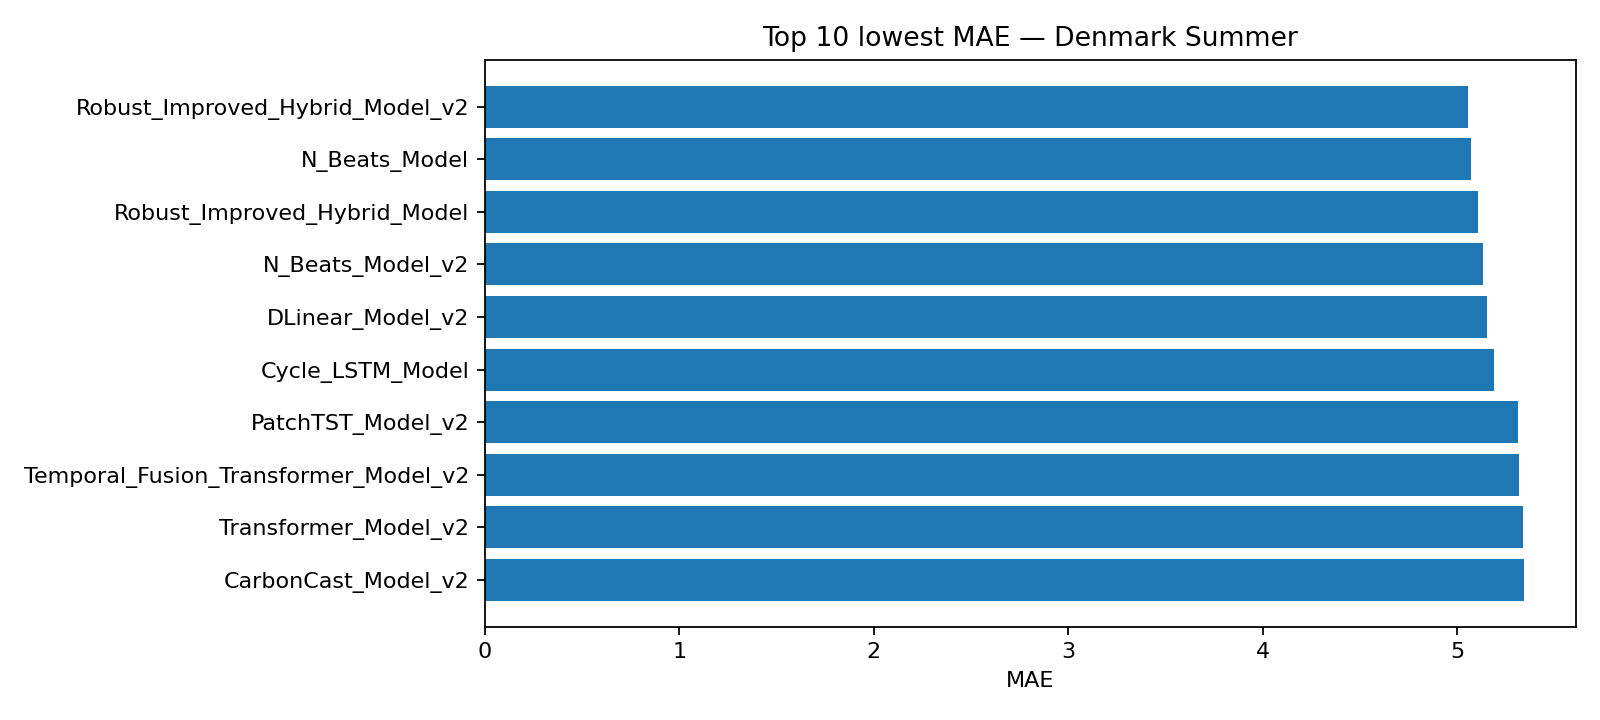
\includegraphics[width=0.48\textwidth]{../Results/Benchmark/top10_mae_Denmark_summer.png}}\hfill
  \subfloat[Denmark Winter]{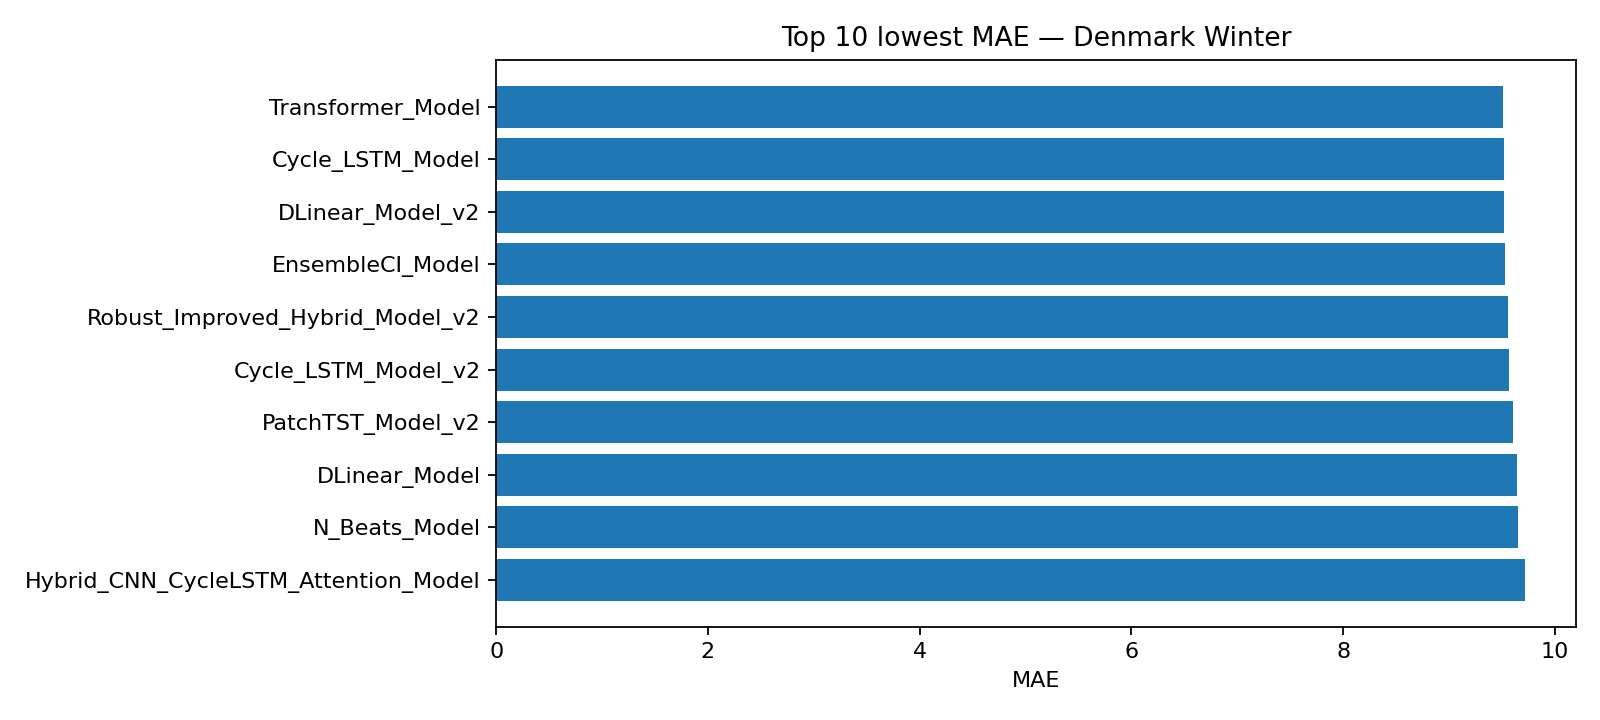
\includegraphics[width=0.48\textwidth]{../Results/Benchmark/top10_mae_Denmark_winter.png}}\\
  \subfloat[Germany Summer]{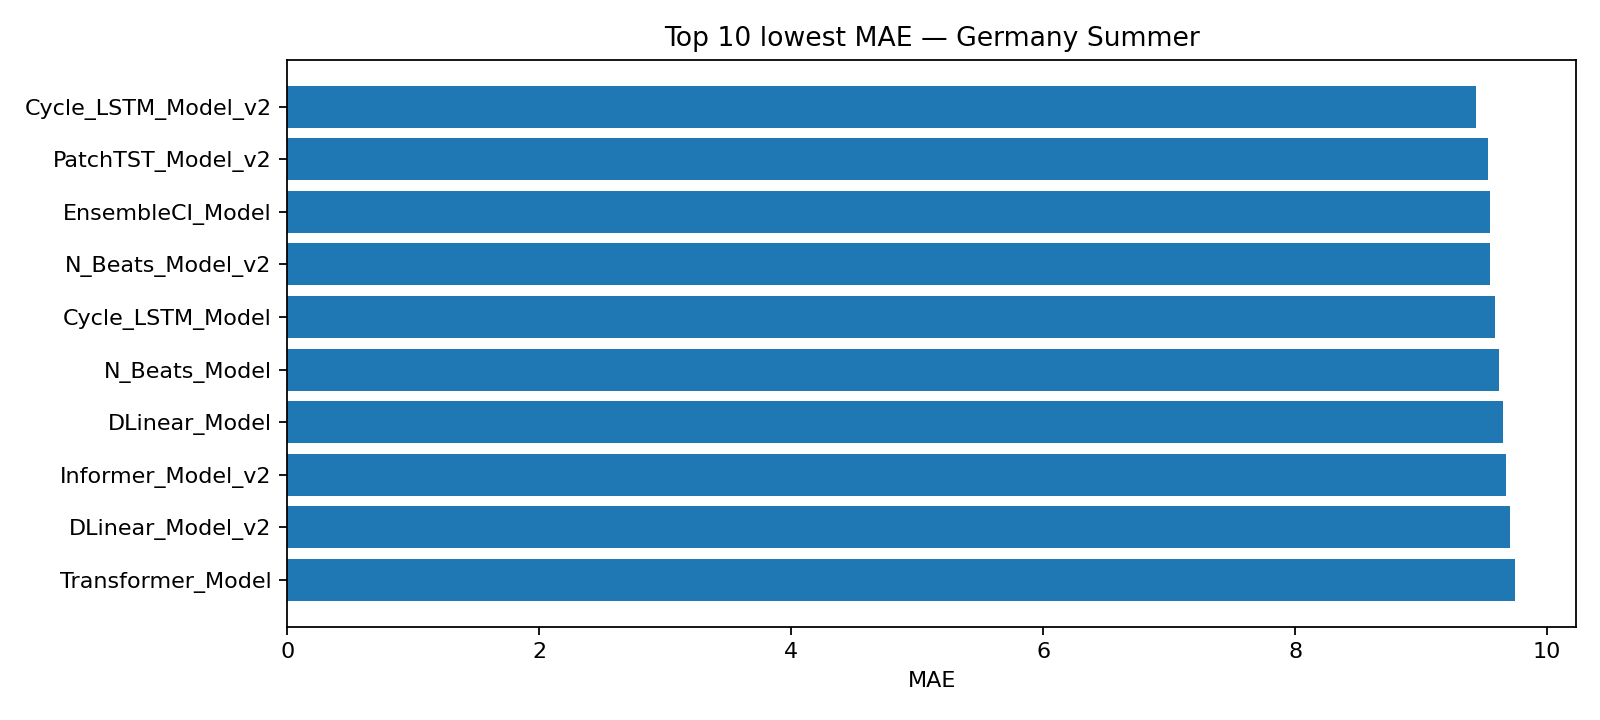
\includegraphics[width=0.48\textwidth]{../Results/Benchmark/top10_mae_Germany_summer.png}}\hfill
  \subfloat[Germany Winter]{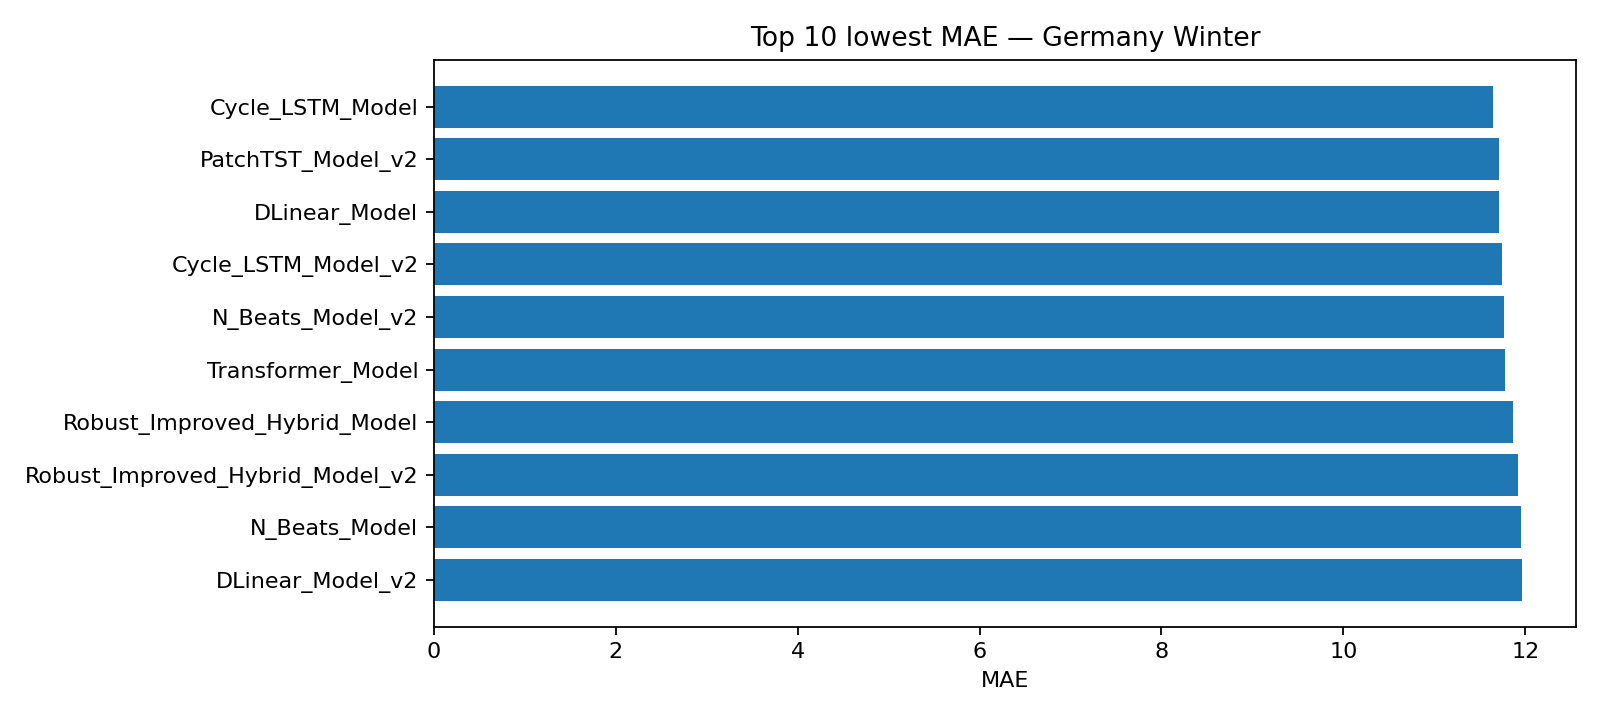
\includegraphics[width=0.48\textwidth]{../Results/Benchmark/top10_mae_Germany_winter.png}}\\
  \subfloat[Hungary Summer]{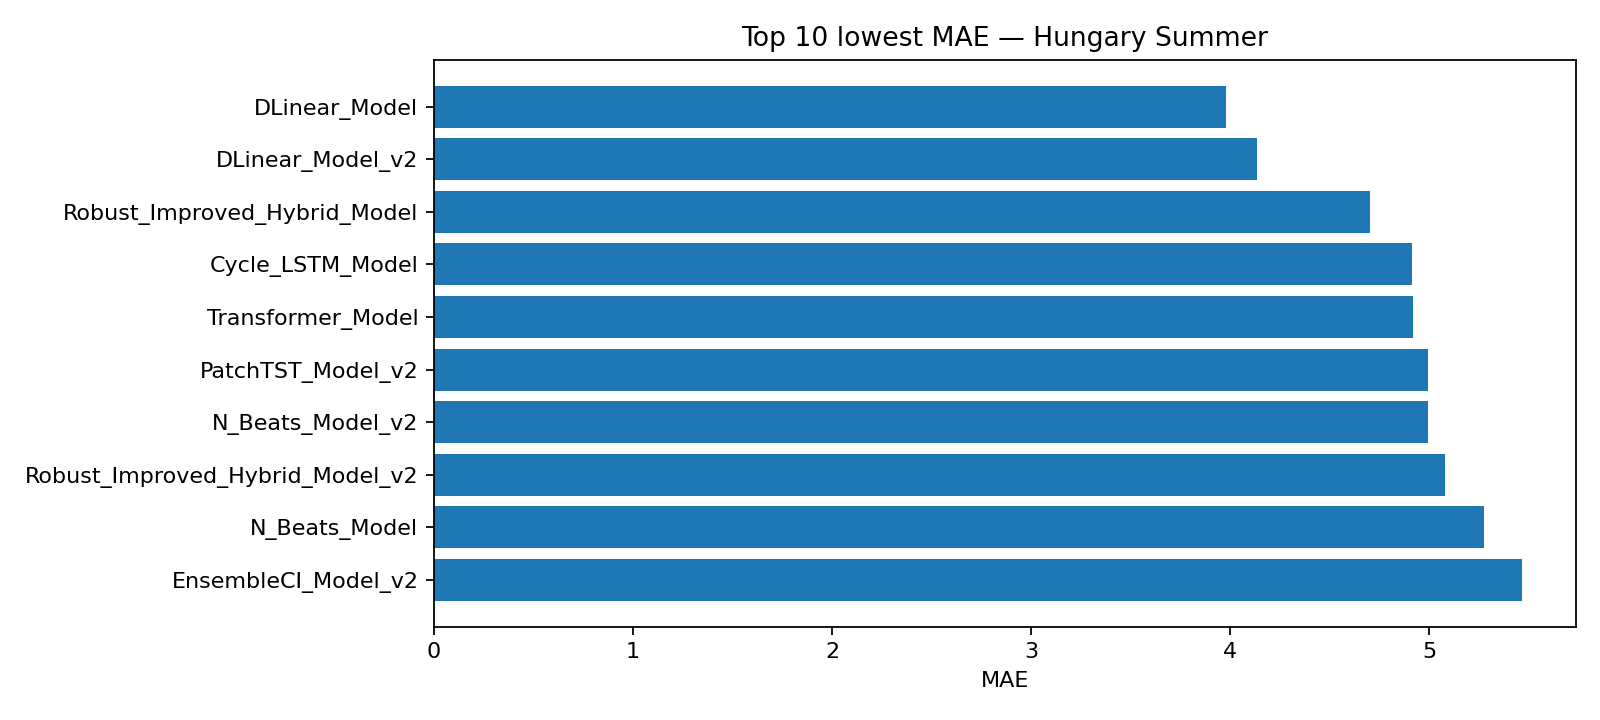
\includegraphics[width=0.48\textwidth]{../Results/Benchmark/top10_mae_Hungary_summer.png}}\hfill
  \subfloat[Hungary Winter]{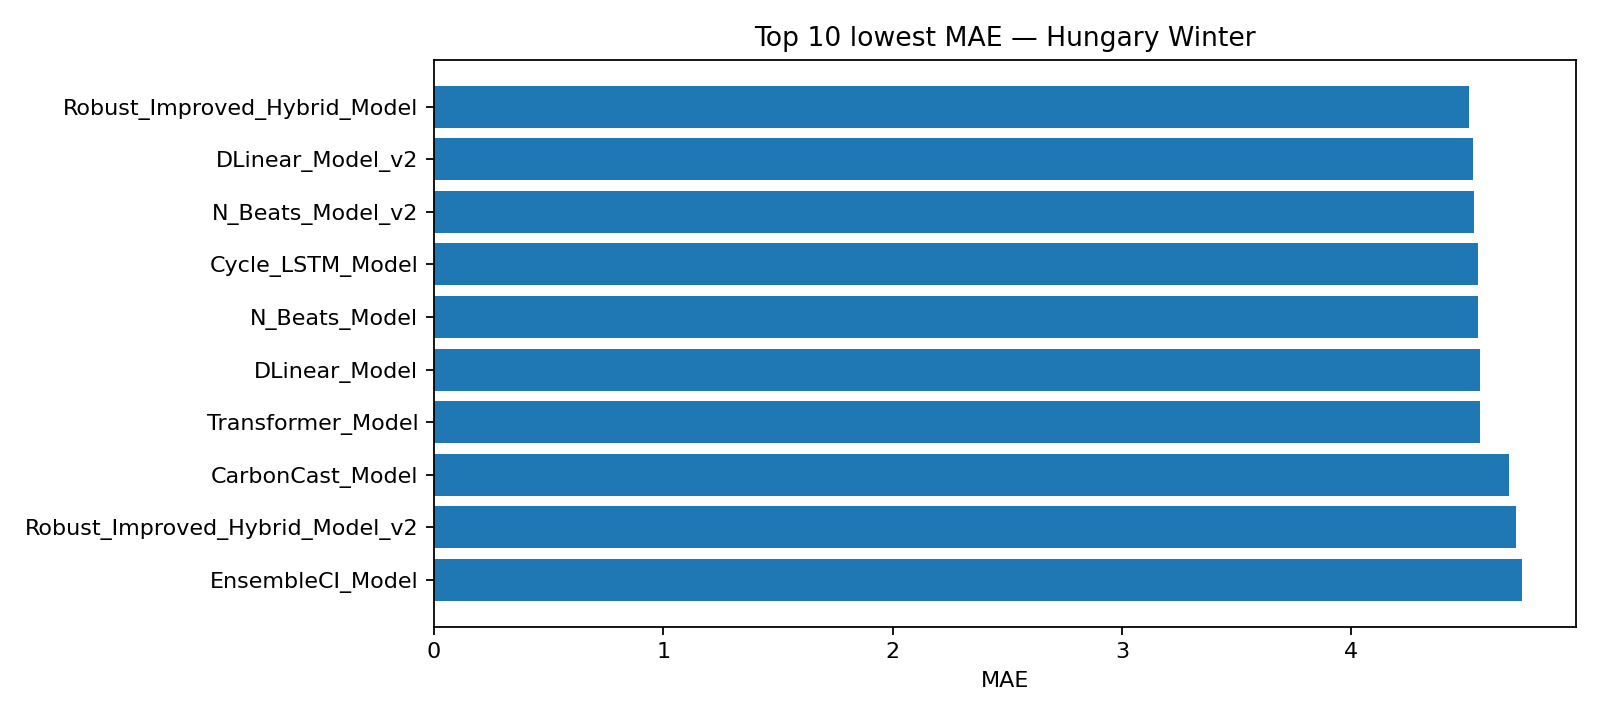
\includegraphics[width=0.48\textwidth]{../Results/Benchmark/top10_mae_Hungary_winter.png}}\\
  \subfloat[Spain Summer]{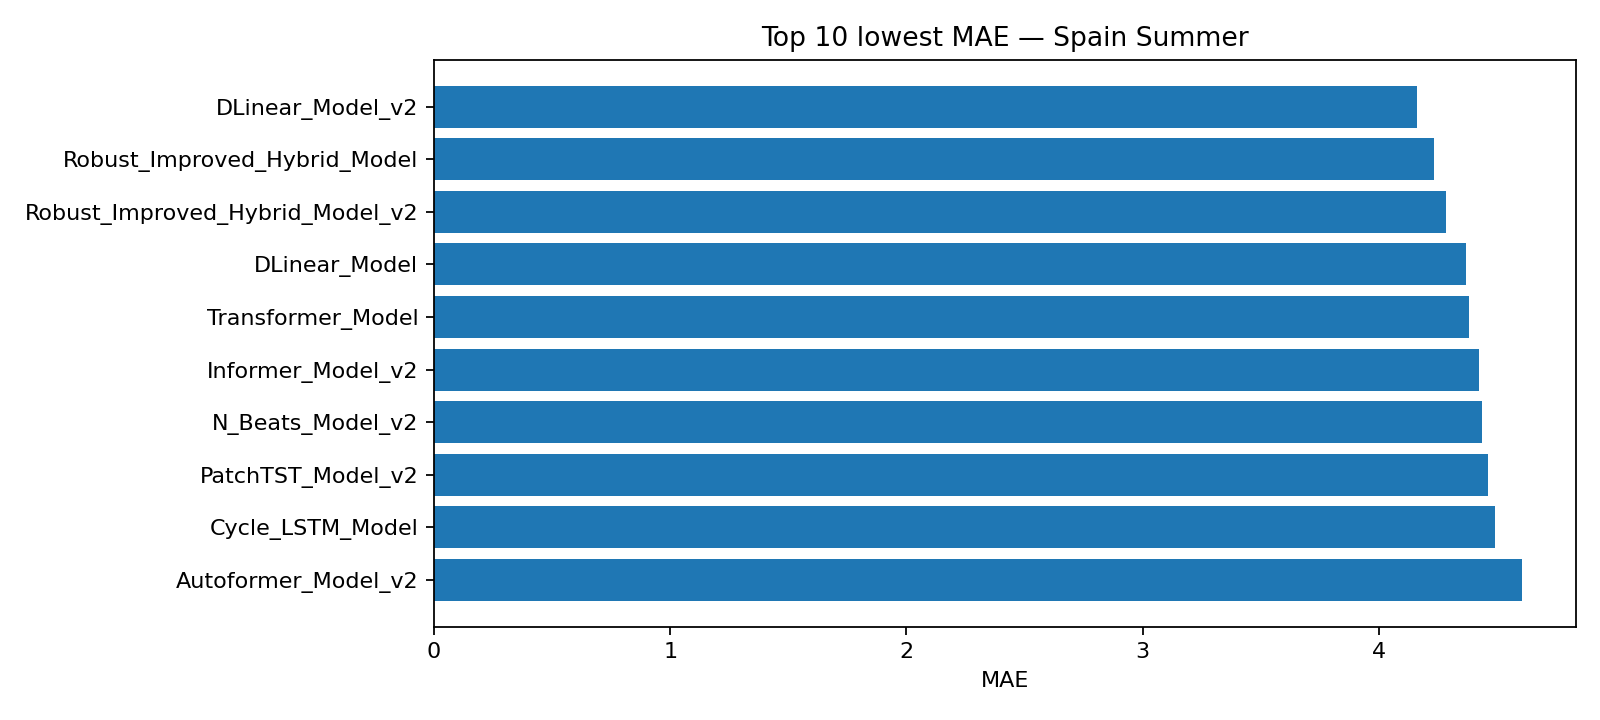
\includegraphics[width=0.48\textwidth]{../Results/Benchmark/top10_mae_Spain_summer.png}}\hfill
  \subfloat[Spain Winter]{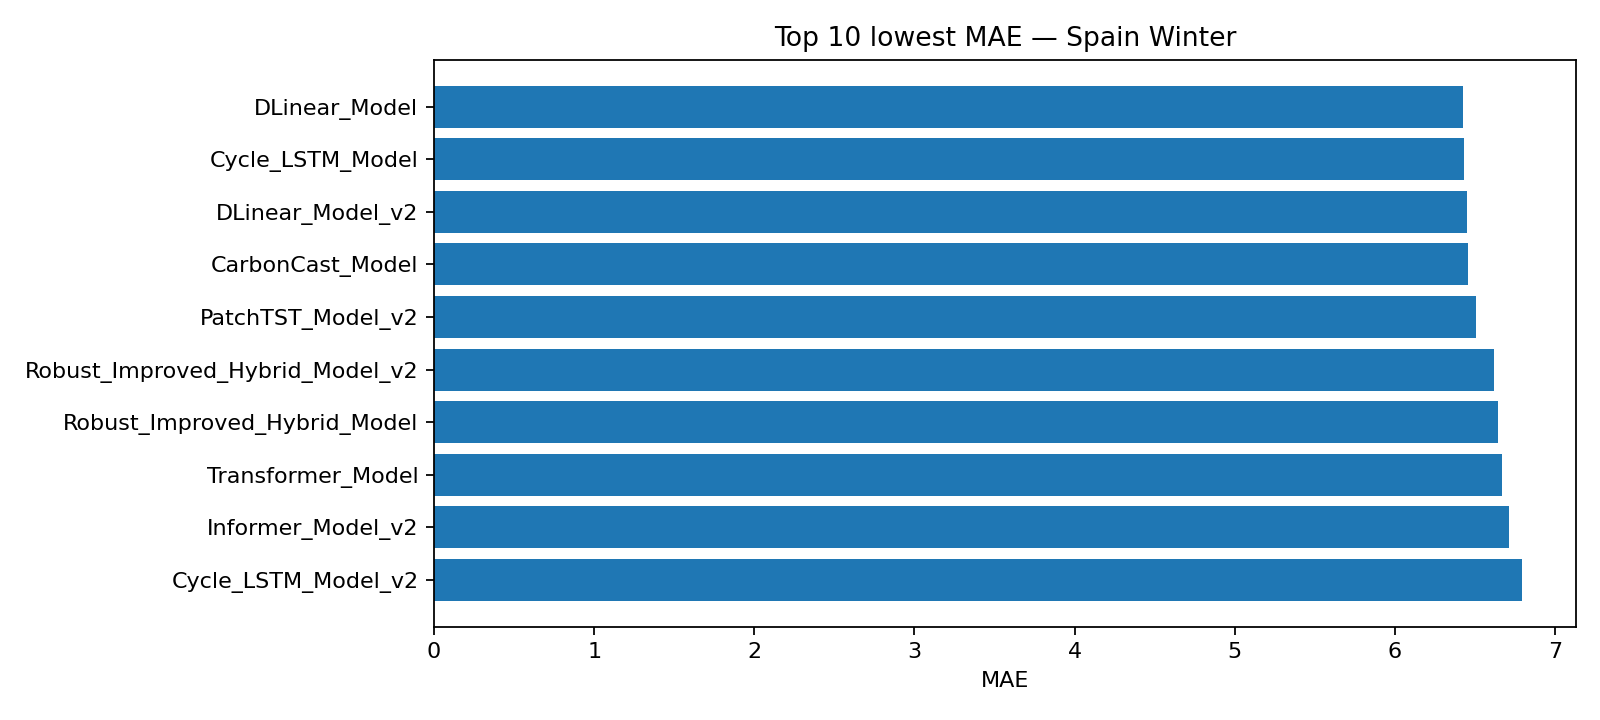
\includegraphics[width=0.48\textwidth]{../Results/Benchmark/top10_mae_Spain_winter.png}}
  \caption{Per-slice Top-10 MAE leaderboards.}
  \label{fig:per_country_top10}
\end{figure*}

% -- Bibliography --
  \appendices
  \section{Reproducibility Commands (Windows PowerShell)}
  Run orchestrations and regenerate benchmark artifacts.
  \begin{verbatim}
  # Full run (both seasons, 4 countries, repeat each twice)
  python .\main.py --season both --countries DE,DK,ES,HU --repeat 2

  # Quick smoke test for DLinear family (summer)
  python .\main.py --season summer --filter DLinear --quick --countries DE,DK,ES,HU

  # Aggregate and plot
  python -m scripts.benchmark

  # Regenerate LaTeX tables for the paper
  python .\Paper\generate_tables.py
  \end{verbatim}

\bibliographystyle{IEEEtran}
\bibliography{references}

\end{document}
